\chapter{Theoretical error in PDFs determination}
\label{ch:th_error}
In order to get an accurate estimate of the uncertainties affecting the Standard Model predictions, theoretical 
errors need to be taken into account. 
For hadron collider processes these are dominated by those due to missing higher order corrections in QCD calculations 
and to PDFs\footnote{From now on we will use the acronyms MHO and MHOU to denote missing higher orders
 and missing higher orders uncertainties respectively.}. 
It is clear how MHOU will also have an affect on the PDFs themselves, being present in the perturbative predictions
of the particular processes used for PDFs determination. Besides from contributing to the overall
size of PDFs uncertainty, MHOU might affect the relative weights different points have in a fit:
points accurately described by the current perturbative predictions (up to NNLO) should weight more
than those poorly described. 
%
As discussed in chapter~\ref{ch:nnpdf_methodology}, present PDFs uncertainties only account for statistical and 
systematic errors affecting the experimental data entering the analysis, and typically do not include any source 
of theory uncertainty.
%
In this chapter, based on Refs.~\cite{AbdulKhalek:2019bux,AbdulKhalek:2019ihb}, we describe how to set up 
a general formalism for the inclusion of theoretical uncertainties in PDFs determinations,
and we specify it to the case of MHOU.

% 
The chapter is structure as follows. In Sec.~\ref{sec:th_err_as_cov} we show how a generic source of theory error 
can be described by means of a covariance matrix; in Sec.~\ref{sec:scale_var} we discuss how, when considering
MHO, such covariance matrix can be constructed using scale variations and a suitable prescription,
which is validated in Sec.~\ref{sec:validation};
in Sec.~\ref{sec:th_error_results} we present a first NLO PDFs set accounting for MHO, and finally in Sec.~\ref{sec:th_error_usage}
we provide instructions on how to use such result in phenomenological applications.


 \section{Theory error as a covariance matrix}
 \label{sec:th_err_as_cov}
 In this section we will show how, by adopting a Bayesian approach and
 assuming a Gaussian prior probability distribution for the true value of the theory, any missing theoretical
 uncertainty can be accounted for by adding a contribution to the experimental covariance matrix used in the PDFs fit.

%
Denoting as $D$ the vector of experimental data entering the analysis and as $\mathcal{T}$ the corresponding vector of 
``true'' unknown values - whose determination is the goal of the experiment - we assume that the experimental results
are Gaussianly distributed about this hypothetical true values $\mathcal{T}$ 
\begin{align}
    \label{eq:conditional_prob}
    P\left(D|\mathcal{T}\right) \propto
    \exp\left(-\frac{1}{2}\left(D-\mathcal{T}\right)^T C^{-1} \left(D-\mathcal{T}\right)\right)\,.
\end{align}
The true values $\mathcal{T}$ are unknown, however we can compute the theory predictions $T$ 
for each experimental data using a theory framework which is 
generally incomplete, for example because it is based on the fixed-order truncation of a perturbative
expansion \footnote{In addition to MHO other effects which could be neglected in the theoretical predictions $T$ are 
higher twist and nuclear effects.}. Furthermore $T$ depend on PDFs, which are evolved up to 
the physical scales of the data using again an incomplete theory. The vectors $\mathcal{T}$ and $T$ would coincide
if the theory were exact and the PDFs were known with certainty.
%
Writing the difference between the true and the actual value of the theory predictions as
\begin{align}
    \label{eq:shifts}
    \Delta = \mathcal{T} - T\,,
\end{align}
we can consider this difference as an additional unknown systematic error, accounting for the incomplete theory.
If we assume, in the same spirit as when estimating experimental systematic, that the true values $\mathcal{T}$ are 
Gaussianly distributed about the theory predictions $T$
\begin{align}
    \label{eq:gaussian_hyp}
    P\left(\mathcal{T}|T\right) \propto 
    \exp\left(-\frac{1}{2}\left(\mathcal{T}-T\right)^T S^{-1} \left(\mathcal{T}-T\right)\right)\,,
\end{align}
then the prior probability distribution of $\Delta$ will be given by
\begin{align}
    P\left(\Delta\right) \propto \exp\left(-\frac{1}{2}\Delta^T S^{-1} \Delta\right)\,. 
\end{align}
Eq.~\eqref{eq:conditional_prob} can be rewritten as
\begin{align}
    P\left(D|\mathcal{T}\right) = P\left(D, \Delta|T\right)  \propto 
    \exp\left(-\frac{1}{2}\left(D - T - \Delta\right)^T C \left(D-T-\Delta\right)\right)\,,   
\end{align}
so that the conditional probability of the data $D$ 
given the theory predictions $T$ can be obtained using the Bayes theorem and marginalizing over $\Delta$ 
\begin{align}
    \label{eq:log_likelihood}
    P&\left(D|T\right) \propto 
    \int d\Delta\, P\left(\Delta\right)P\left(D, \Delta|T\right)  \nonumber\\
    &=\int d\Delta\, \exp\left(-\frac{1}{2}\left(D - T - \Delta\right)^T C^{-1} \left(D-T-\Delta\right) 
    -\frac{1}{2}\Delta^T S^{-1} \Delta \right) \nonumber \\
    &\propto \exp\left(-\frac{1}{2} \left(D-T\right)^T\left(C + S\right)^{-1} \left(D-T\right) \right)\,,
\end{align}
where in the last line we have performed explicitly the Gaussian integral over $\Delta$.
Eq.~\eqref{eq:log_likelihood} defines the likelihood which is usually minimized in a Gaussian fit and shows how
theoretical uncertainties can be treated simply as another form of experimental systematic: 
it is an additional uncertainty to be taken into account when trying to find the truth from the data
using a specific theory setting, and it can be accounted for by mean of an additional contribution $S$ to
the experimental covariance matrix $C$.

%
The problem is then to estimate the theory covariance matrix $S$. The Gaussian hypothesis Eq.~\eqref{eq:gaussian_hyp}
implies that 
\begin{align}
    \label{eq:def_th_cov_0}
    \int d\mathcal{T} \, P\left(\mathcal{T}|T\right) \left(\mathcal{T}-T\right)_i \left(\mathcal{T}-T\right)_j = 
    \langle \Delta_i \,\Delta_j \rangle = S_{ij}\,,
\end{align}
showing how in general we need to estimate the shifts $\Delta_i$ defined in Eq.~\eqref{eq:shifts}, in a way that takes into account
the theoretical correlations between different points within the same dataset, between different datasets
measuring the same physical process and between datasets corresponding to different processes
\footnote{Unlike experimental correlations, theory correlations will be present even for entirely different processes,
through the universal parton distributions, which all share the same theory for DGLAP evolution.}.

\section{MHOU from scale variations}
\label{sec:scale_var}
The most commonly used method to estimate the theory corrections due to MHO is scale variations. 
In the following we briefly revise its key ingredients and fix the conventions and terminology used in this work.
For simplicity we will discuss the case of electroproduction processes, like DIS, but the same argument
can be used to obtain expressions for a generic hadronic process. 
We refer to Ref.~\cite{AbdulKhalek:2019ihb} for a complete and formal discussion of the topic.

%
Considering the problem of PDFs determination and remembering the factorized expression
for high-energy processes cross-sections, there are two independent source of MHOU: the 
perturbative expression of the partonic cross-section and the perturbative expression of the 
anomalous dimensions that determine the evolution of parton distributions.
These will be associated with two independent unphysical scales, which here will be denoted as renormalization scale
$\mu_r$ and factorization scale $\mu_f$.
Using RG equations for hard cross-sections and for PDFs it is possible to obtain an estimate of the MHOU
by varying independently the two unphysical scales entering the problem.

Considering a generic structure function, 
denoting as $\overline{F}$ the corresponding scale-dependent theory prediction\footnote{The structure 
function $\overline{F}$ depend on $\mu_r^2$ and $\mu_f^2$ in the sense of the RG
equation: the dependence on unphysical scales cancels order by order, and the residual dependence can
be used to estimate the MHOU.}
we have 
\begin{align}
\label{eq:scale_var_F_Q}
    \overline{F}\left(Q^2,\mu_r^2, \mu_f^2\right) &= 
    \overline{C}\left(\alpha_s\left(\mu_r^2\right),\frac{\mu_r^2}{Q^2}\right)\otimes 
    q\left(\alpha_s\left(\mu_f^2\right),\frac{\mu_f^2}{Q^2}\right)\,. 
\end{align}
Following the notations of Ref.~\cite{AbdulKhalek:2019ihb}, we introduce the variables
$t = \log Q^2/\Lambda^2$, $k_r = \log \mu_r^2/Q^2$ and $k_f = \log \mu_f^2/Q^2$ so that Eq.~\eqref{eq:scale_var_F_Q}
can be written as 
\begin{align}
    \label{eq:scale_var_F}
    \overline{F}\left(k_r, k_f\right)=
    \overline{C}\left(\alpha_s\left(t+k_r\right),k_r\right)\otimes \overline{q}\left(\alpha_s\left(t+k_f\right),k_f\right)\,.
    \end{align}
In the following, we will use the notations $\overline{F}$, $\overline{C}$ and $\overline{q}$ to denote 
structure functions, Wilson coefficients and PDFs evaluated at the generic scale $\mu_r$ and $\mu_f$.
When setting such scales equal to the physical one $Q$, namely when either $k_r=0$ or $k_f=0$ we define
\begin{align}
    \label{eq:central_scale}
    &F\left(0,0\right) \equiv \overline{F}\left(0, 0\right)\,, \nonumber\\
    &C\left(t\right)   \equiv \overline{C}\left(\alpha_s\left(t\right),0\right)\,,\\
    &q\left(t\right)   \equiv \overline{q}\left(\alpha_s\left(t\right),0\right)\,. \nonumber
\end{align}
In order to estimate the MHOU due to the truncation of the perturbative expansion of the coefficient function 
$\overline{C}$ we can fix a specific renormalization scheme and keep $\mu_f = Q$, but varying
the renormalization scale $\mu_r^2$ used in the computation of the coefficient function itself.
The scale-dependent structure function $\overline{F}$ will then be given by
\begin{align}
    \overline{F}\left(Q^2,\mu_r^2\right) = 
    \overline{C}\left(\alpha_s\left(\mu_r^2\right),\frac{\mu_r^2}{Q^2}\right)\otimes q\left(Q^2\right) 
    &=\overline{C}\left(\alpha_s\left(t+k_r\right),k_r\right)\otimes q\left(t\right)\,.
\end{align}
Using the RG invariance of the physical cross section
\begin{align}
    \label{eq:RG_invariance}
    \mu_r^2\frac{d}{d\mu_r^2}\overline{F}\left(Q^2,\mu_r^2\right) = \frac{d}{dk_r}\overline{F}\left(t,k_r\right)=0\,,
\end{align}
it is easy to show that
the renormalization scale dependent Wilson coefficients $\overline{C}$ can be written as
\begin{align}
    \label{eq:wilson_coeff_scale_var}
    \overline{C}\left(\alpha_s\left(t+k_r\right),k_r\right) =
    C\left(t+k_r\right) &-  k\frac{d}{dt}C\left(t+k_r\right) 
    + \frac{1}{2} k_r^2\, \frac{d^2}{dt^2}C\left(t+k_r\right) + ...
\end{align}
where according to Eq.~\eqref{eq:central_scale} $C\left(t\right) = \overline{C}\left(\alpha_s\left(t\right),0\right)$.
In other words, thanks to the RG invariance we can write the renormalization scale dependent Wilson coefficients
at a generic scale $\mu_r$ in terms of their values at the physical scale $\mu_r=Q$.
The log derivatives appearing in Eq.~\eqref{eq:wilson_coeff_scale_var} can be easily evaluated using the 
perturbative expression of $C$ 
\begin{align}
    C\left(t\right) = 
    c_0 + \alpha_s\left(t\right)c_1 + \alpha_s^2\left(t\right)c_2 + \alpha_s^3\left(t\right)c_3 + ...\,,
\end{align}
and of the $\beta$ function expansion Eq.~\eqref{eq:beta_function_expansion} getting
\begin{align}
    \label{eq:scale_varied_wilson_coeff}
    \overline{C}&\left(\alpha_s\left(t+k_r\right),k_r\right) = c_0 
    + \alpha_s\left(t+k_r\right)c_1 + \alpha_s^2\left(t+k_r\right)\left(c_2 + k_r\beta_0 c_1\right) \nonumber \\
    &+ \alpha_s^3\left(t+k_r\right)\left(c_3 + k_r\beta_0\left(\beta_1c_1 +2c_2 - k_r\beta_0 c_1\right)\right)\, + ...
\end{align} 

%
In the same way, starting again from Eq.~\eqref{eq:scale_var_F}, in order to get the 
scaled varied PDF we can fix $\mu_r=Q$
and vary the scale $\mu_f$ at which the PDFs are evaluated. Setting $\mu_r=Q$ we get 
\begin{align}
    \overline{F}\left(Q^2,\mu_f^2\right)& = 
    C\left(\alpha_s\left(Q^2\right)\right)\otimes 
    \overline{q}\left(\alpha_s\left(\mu_f^2\right),\frac{\mu_f^2}{Q^2}\right) \nonumber \\
    &=C\left(t\right)\otimes \overline{q}\left(\alpha_s\left(t+k_f\right),k_f\right)\,,
\end{align}
and using the RG invariance Eq.~\eqref{eq:RG_invariance} with respect to $\mu_f$ we get 
\begin{align}
    \label{eq:scale_vare_pdf_1}
    \overline{q}\left(\alpha_s\left(t+k_f\right),k_f\right) = q\left(t+k_f\right) &-  k_f\frac{d}{dt}q\left(t+k_f\right) 
    + \frac{1}{2} k_f^2\,\frac{d^2}{dt^2}q\left(t+k_f\right) + ...
\end{align}
where in analogy with what done for the Wilson coefficients we have defined 
$q\left(t\right) \equiv \overline{q}\left(\alpha_s\left(t\right),0\right)$.
Using the evolution equation\footnote{for simplicity, in
this section all the argument is presented implicitly assuming a Mellin space formalism, so that
convolutions are replaced by ordinary products.}
\begin{align}
    \frac{d}{d\mu_f^2}\, q\left(\mu_f^2\right) = \gamma\left(\alpha_s\left(\mu_f^2\right)\right)q\left(\mu_f^2\right)\,,
\end{align}
Eq.~\eqref{eq:scale_vare_pdf_1} can be rewritten as 
\begin{align}
    \label{eq:scale_var_pdf_2}
    \overline{q}\left(\alpha_s\left(t+k_f\right),k_f\right) = &q\left(t+k_f\right) - k\gamma q\left(t+k_f\right) \nonumber\\
    &+ \frac{1}{2}k^2\left(\gamma^2 + \frac{d}{dt}\gamma\right)q\left(t+k_f\right) + ...\,,
\end{align}
which can be further simplified using the perturbative expansion of the anomalous dimension
and the expression for the $\beta$ function\footnote{In Ref.~\cite{AbdulKhalek:2019ihb} it is explicitly shown that an 
alternative way of obtaining Eq.~\eqref{eq:scale_var_pdf_2} consists in varying the renormalization scale of the anomalous dimension.
MHOU due to PDFs evolution can therefore be estimated varying either the PDFs scale or the scale of the anomalous dimension.}.

%
Eqs.~\eqref{eq:scale_varied_wilson_coeff},\eqref{eq:scale_var_pdf_2} allow to easily perform scale variations for a single process,
varying independently the two unphysical scales $\mu_r$ and $\mu_f$.
In particular, they allow to obtain scaled varied coefficient functions and PDFs in terms of the corresponding values 
computed at the physical scale $Q$. 
Considering a specific process involved in the PDFs fit, one can, for example, perform scale variation in the range
$|k_r|, |k_f| < \log 4$, obtaining the scale varied cross section $\overline{F}\left(k_r, k_f\right)$.
When considering hadronic processes,
the same arguments presented above can be used to obtain a formula similar to the one of Eq.~\eqref{eq:scale_varied_wilson_coeff},
as shown in Ref.~\cite{AbdulKhalek:2019ihb}.

%
We now consider a situation where we have $p$ different types of processes (like for example electroproduction processes, 
hadronic processes, jets ...) 
\[\pi_a = \{i_a\}\,, \,\,\,\,\,\,\,\, a = 1,...,p\,,\] 
where $i_a$ labels the datapoints belonging to the $a$-th process.
Each of them is characterized by a factorization scale $\mu_f$ (associated to the universal PDFs) and a renormalization scale 
$\mu_{r_a}$ (associated with the hard coefficient functions).
Given the $i$-th point of the $a$-th process $F_{i_a}$, we define the corresponding shift $\Delta_{i_a}$ as 
\begin{align}
    \Delta_{i_a}\left(k_f,k_{r_a}\right) \equiv \overline{F}_{i_a}\left(k_f, k_{r_a}\right) - F_{i_a}\left(0, 0\right)\,,
\end{align}
where we assume that all scale variations can be performed in the same range $|k_{r_a}|, |k_f| < \log 4$.
In practice, for each scale three points can be sampled, corresponding to $k = 0, \pm \log 4$.
Note that since the PDFs are universal but the coefficient functions are process dependent,
when considering two different processes the scale variations of $k_{r}$ will be totally independent 
while those of $k_f$ will be correlated between different processes. 
In other words, because of PDFs universality the relation between the physical scale of each process (whatever that is)
and the factorization scale $\mu_f$ is the same for all the processes.

According to Eq.~\eqref{eq:def_th_cov_0}, the theory covariance matrix is then constructed by averaging
outer products of the shifts over points in the space of scales 
\begin{align}
    \label{eq:th_cov_matrix_1}
    S_{ij} = N \sum_V \Delta_{i_a}\left(k_f,k_{r_a}\right) \Delta_{j_b}\left(k_f,k_{r_b}\right)\,,
\end{align} 
where $i_a \in \pi_a$ and $j_b \in \pi_b$ indicate two data points possibly corresponding to different
processes $\pi_a$ and $\pi_b$, $V$ is the set of scale points to be summed over and $N$ is a normalization factor.
Note that from this definition it follows immediately that the
theory covariance matrix is positive definite: considering a real vector $v_i$, from Eq.~\eqref{eq:th_cov_matrix_1}
we have
\begin{align}
    \sum_{ij} v_i S_{ij} v_j = N \sum_{V}\left(\sum_i v_i \Delta_i\right)^2 \geq 0\,.
\end{align}

%
Different prescriptions for the theory covariance matrix definition can be adopted, characterized by a different
set of combination of scales which are summed over in Eq.~\eqref{eq:th_cov_matrix_1}.
Here we will discuss results for the so called 9-points prescriptions, referring to the original publication 
Ref.~\cite{AbdulKhalek:2020jut} for more details about alternative possibilities.
For simplicity, let's first consider the theory covariance matrix entries corresponding to 
a couple of points belonging to the same process. In this case there are at most two independent scales to be varied,
corresponding to the renormalization and factorization scales $k_r$ and $k_f$.
In the 9-points prescription $k_r$ and $k_f$ are varied completely independently, getting the 8 + 1 points in the 
scales space reported in Fig.~\ref{fig:symmetricPrescriptions} (left), where the +1 refers to the trivial 
point $k_r=k_f=0$ for which the shift $\Delta_i$ vanishes.
The normalization factor appearing in Eq.~\eqref{eq:th_cov_matrix_1}
is determined by averaging over the number of points associated with the variation of each scale,
and adding the contributions from variation of independent scales.
So in the case of the 9-points prescriptions we have 8 points and 2 independent scales, 
giving a normalization factor $N=1/4$. The corresponding theory covariance matrix entries read
\begin{equation}
    \label{9S}
    \begin{split}
        S^{(\rm 9pt)}_{ij} = \frac{1}{4}\{ &\Delta_i^{+0} \Delta_j^{+0} + \Delta_i^{-0}\Delta_j^{-0}
                                + \Delta_i^{0+} \Delta_j^{0+} + \Delta_i^{0-}\Delta_j^{0-} \\
                                + &\Delta_i^{++}\Delta_j^{++} + \Delta_i^{+-} \Delta_j^{+-}
                                + \Delta_i^{-+}\Delta_j^{-+} + \Delta_i^{--} \Delta_j^{--} \} \,,
    \end{split}                            
\end{equation}
where the superscripts $+,-,0$ denote the different variations of $k_r$ and $k_f$ defining the shift. 
Such construction can be generalized to the case of couples of
points belonging to two different processes $\pi_1$ and $\pi_2$. The set $V$ now involves 
possible variations of three scales $k_f,k_{r_1}, k_{r_2}$, represented in the right plot 
of Fig.~\ref{fig:symmetricPrescriptions}.
Again, varying such scales independently and accounting for the corrects normalization factors,
Eq.~\eqref{9S} can be generalized to the off-diagonal blocks of the theory covariance matrix, giving
\begin{equation}\label{9M}
\begin{split}
    S^{(\rm 9pt)}_{i_1j_2} =
    \frac{1}{24}\{&2\big(\Delta_{i_1}^{+0}+\Delta_{i_1}^{++}
    + \Delta_{i_1}^{+-}\big) \big(\Delta_{j_2}^{+0} +
    \Delta_{j_2}^{++} + \Delta_{j_2}^{+-} \big) \\ 
            + &2\big(\Delta_{i_1}^{-0} + \Delta_{i_1}^{-+} +
            \Delta_{i_1}^{--}\big)\big(\Delta_{j_2}^{-0} +
            \Delta_{j_2}^{-+} + \Delta_{j_2}^{--} \big) \big\}\\ 
            + &3\big(\Delta_{i_1}^{0+}+ \Delta_{i_1}^{0-}\big)\big(\Delta_{j_2}^{0+} + \Delta_{j_2}^{0-} \big)\}.
\end{split}            
\end{equation}

\begin{figure}[t]
    \centering
    {\begin{tikzpicture}
    \draw[->] (-1.5,0) -- (1.5,0);
    \draw[->] (0,-1.5) -- (0,1.5);
    \filldraw[black] (0,0) circle (2pt);
    \filldraw[black] (-1,0) circle (2pt);
    \filldraw[black] (0,-1) circle (2pt);
    \filldraw[black] (1,0) circle (2pt);
    \filldraw[black] (0,1) circle (2pt);
    \filldraw[black] (-1,-1) circle (2pt);
    \filldraw[black] (1,-1) circle (2pt);
    \filldraw[black] (-1,1) circle (2pt);
    \filldraw[black] (1,1) circle (2pt);
    \node at (0.5,1.5) {$\kappa_r$};
    \node at (1.9,0) {$\kappa_f$};
    \end{tikzpicture}}
    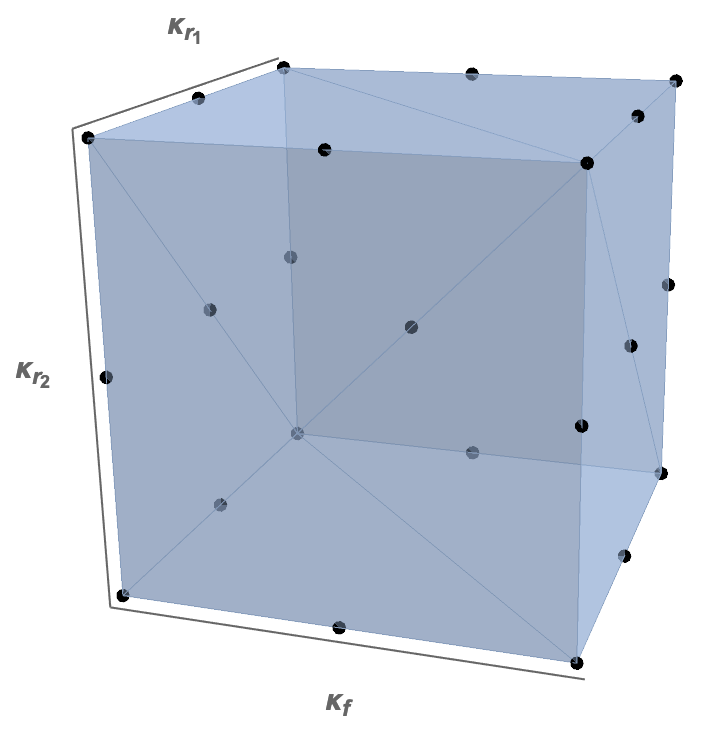
\includegraphics[scale=0.29]{9pt_3D.png}
    \begin{caption}{9-points prescription for a single process (left) and for two different processes $\pi_1$
        and $\pi_2$, indicating
        the sampled values for the factorization scale $\kappa_f$ and 
        renormalization scale $\kappa_r$. Figure from Ref.~\cite{AbdulKhalek:2019ihb}.
    \label{fig:symmetricPrescriptions}
      }
    \end{caption}
    \end{figure}

    \section{Construction and validation of a theory covariance matrix}
    \label{sec:validation}
    In this section we determine the theory covariance matrix at NLO using Eqs.~\eqref{9S}, \eqref{9M}
    and we validate it against the known NNLO results.
    As input datasets, we use the same NNPDF3.1 baseline given in Tab.~\ref{tab:experiments_chi2} with two minor differences:
    the value of the lower kinematic cut has been increased from $Q^2_{min} = 2.69 \,\,\text{GeV}^2$ to $13.96 \,\, \text{GeV}^2$
    in order to ensure the validity of the perturbative QCD expansion when scales are varied downwards, 
    and the HERA $F^b_2$ and fixed-target Drell-Yan cross-sections have been removed, 
    for technical reasons related to difficulties in implementing scale variation. 
    In total we then have $N_{dat} = 2819$ data points.
    As seen in the previous section, we assume that renormalization scale variation is fully correlated within 
    a given process, but uncorrelated between different processes.
    Having defined the input experimental data it is then necessary to define what we mean by ``process'' and
    divide the input dataset accordingly.
    Our categorization, summarized in Tab.~\ref{eq:expclassification}, involves five distinct processes:  charged-current (CC)
    and neutral-current (NC) deep-inelastic scattering (DIS),
    Drell–Yan (DY) production of gauge bosons (invariant mass,
    transverse momentum and rapidity distributions), single-jet
    inclusive and top pair production cross-sections.
    Note that such categorization requires and educated guess as to which theory computations share the same higher order
    corrections, and different choices might be done. 
    We consider the one presented here to be sufficient for a first study. 
    %
    In order to evaluate the theory covariance matrix $S_{ij}$, it is necessary
    to be able to evaluate both DIS structure functions and hadronic
    cross-sections for a range of values of the factorization
    and renormalization scales, i.e.for $k_f \neq  0$ and $k_r \neq 0$.
    %
    In this case, the entries of the NLO theory covariance matrix have been 
    constructed
    by means of the {\tt ReportEngine} software~\cite{zahari_kassabov_2019_2571601}
    taking the
    scale-varied NLO theory cross-sections $\overline{F}_i(k_f,k_r)$  as input.
    %
    These are provided 
    by {\tt APFEL}~\cite{Bertone:2013vaa} for the DIS structure functions
    and by {\tt APFELgrid}~\cite{Bertone:2016lga} combined with
    {\tt APPLgrid}~\cite{Carli:2010rw} for the hadronic
    cross-sections.

    \begin{table}[t]
        \centering
        \renewcommand*{\arraystretch}{1.3}
        \begin{tabular}{|c|c|}
          \hline
          Process Type  & Datasets \\
          \hline
          DIS NC  &   NMC, SLAC, BCDMS, HERA NC \\
          DIS CC  &   NuTeV, CHORUS, HERA CC \\
          DY  & CDF, D0, ATLAS, CMS, LHCb ($y$, $p_T$, $M_{ll}$) \\
          JET  & ATLAS, CMS inclusive jets \\
          TOP  & ATLAS, CMS total+differential cross-sections \\
          \hline
        \end{tabular}
        \caption{\label{eq:expclassification}
         Classification of  datasets into  process types.
        }
    \end{table}
    %
    In order to get an idea of the structure of the theory-induced correlations,
    in Fig.~\ref{fig:covmats} we compare the experimental correlation matrix, given by
    \begin{align}
        \rho^{(C)}_{ij} = \frac{C_{ij}}{\sqrt{C_{ii}}\sqrt{C_{jj}}}\,,
    \end{align}
    with the corresponding combined experimental and theoretical correlation matrix
    \begin{align}
        \rho^{(C+S)}_{ij} = \frac{\left(C+S\right)_{ij}}{ \sqrt{\left(C+S\right)_{ii}} \sqrt{\left(C+S\right)_{jj}} }\,.
    \end{align}
    By inspection of Fig.~\ref{fig:covmats} large positive correlations within individual experiments along 
    the diagonal blocks are apparent, particularly evident for DIS NC and DY data.
    Within the same process there are large correlations between experiments for the DY, jets and top datapoints 
    and large anticorrelations for the DIS NC points. Correlations and anticorrelations between different processes,
    despite being present thanks to PDFs universality, are generally weaker.

    \begin{figure}[t!]
    \begin{center}
        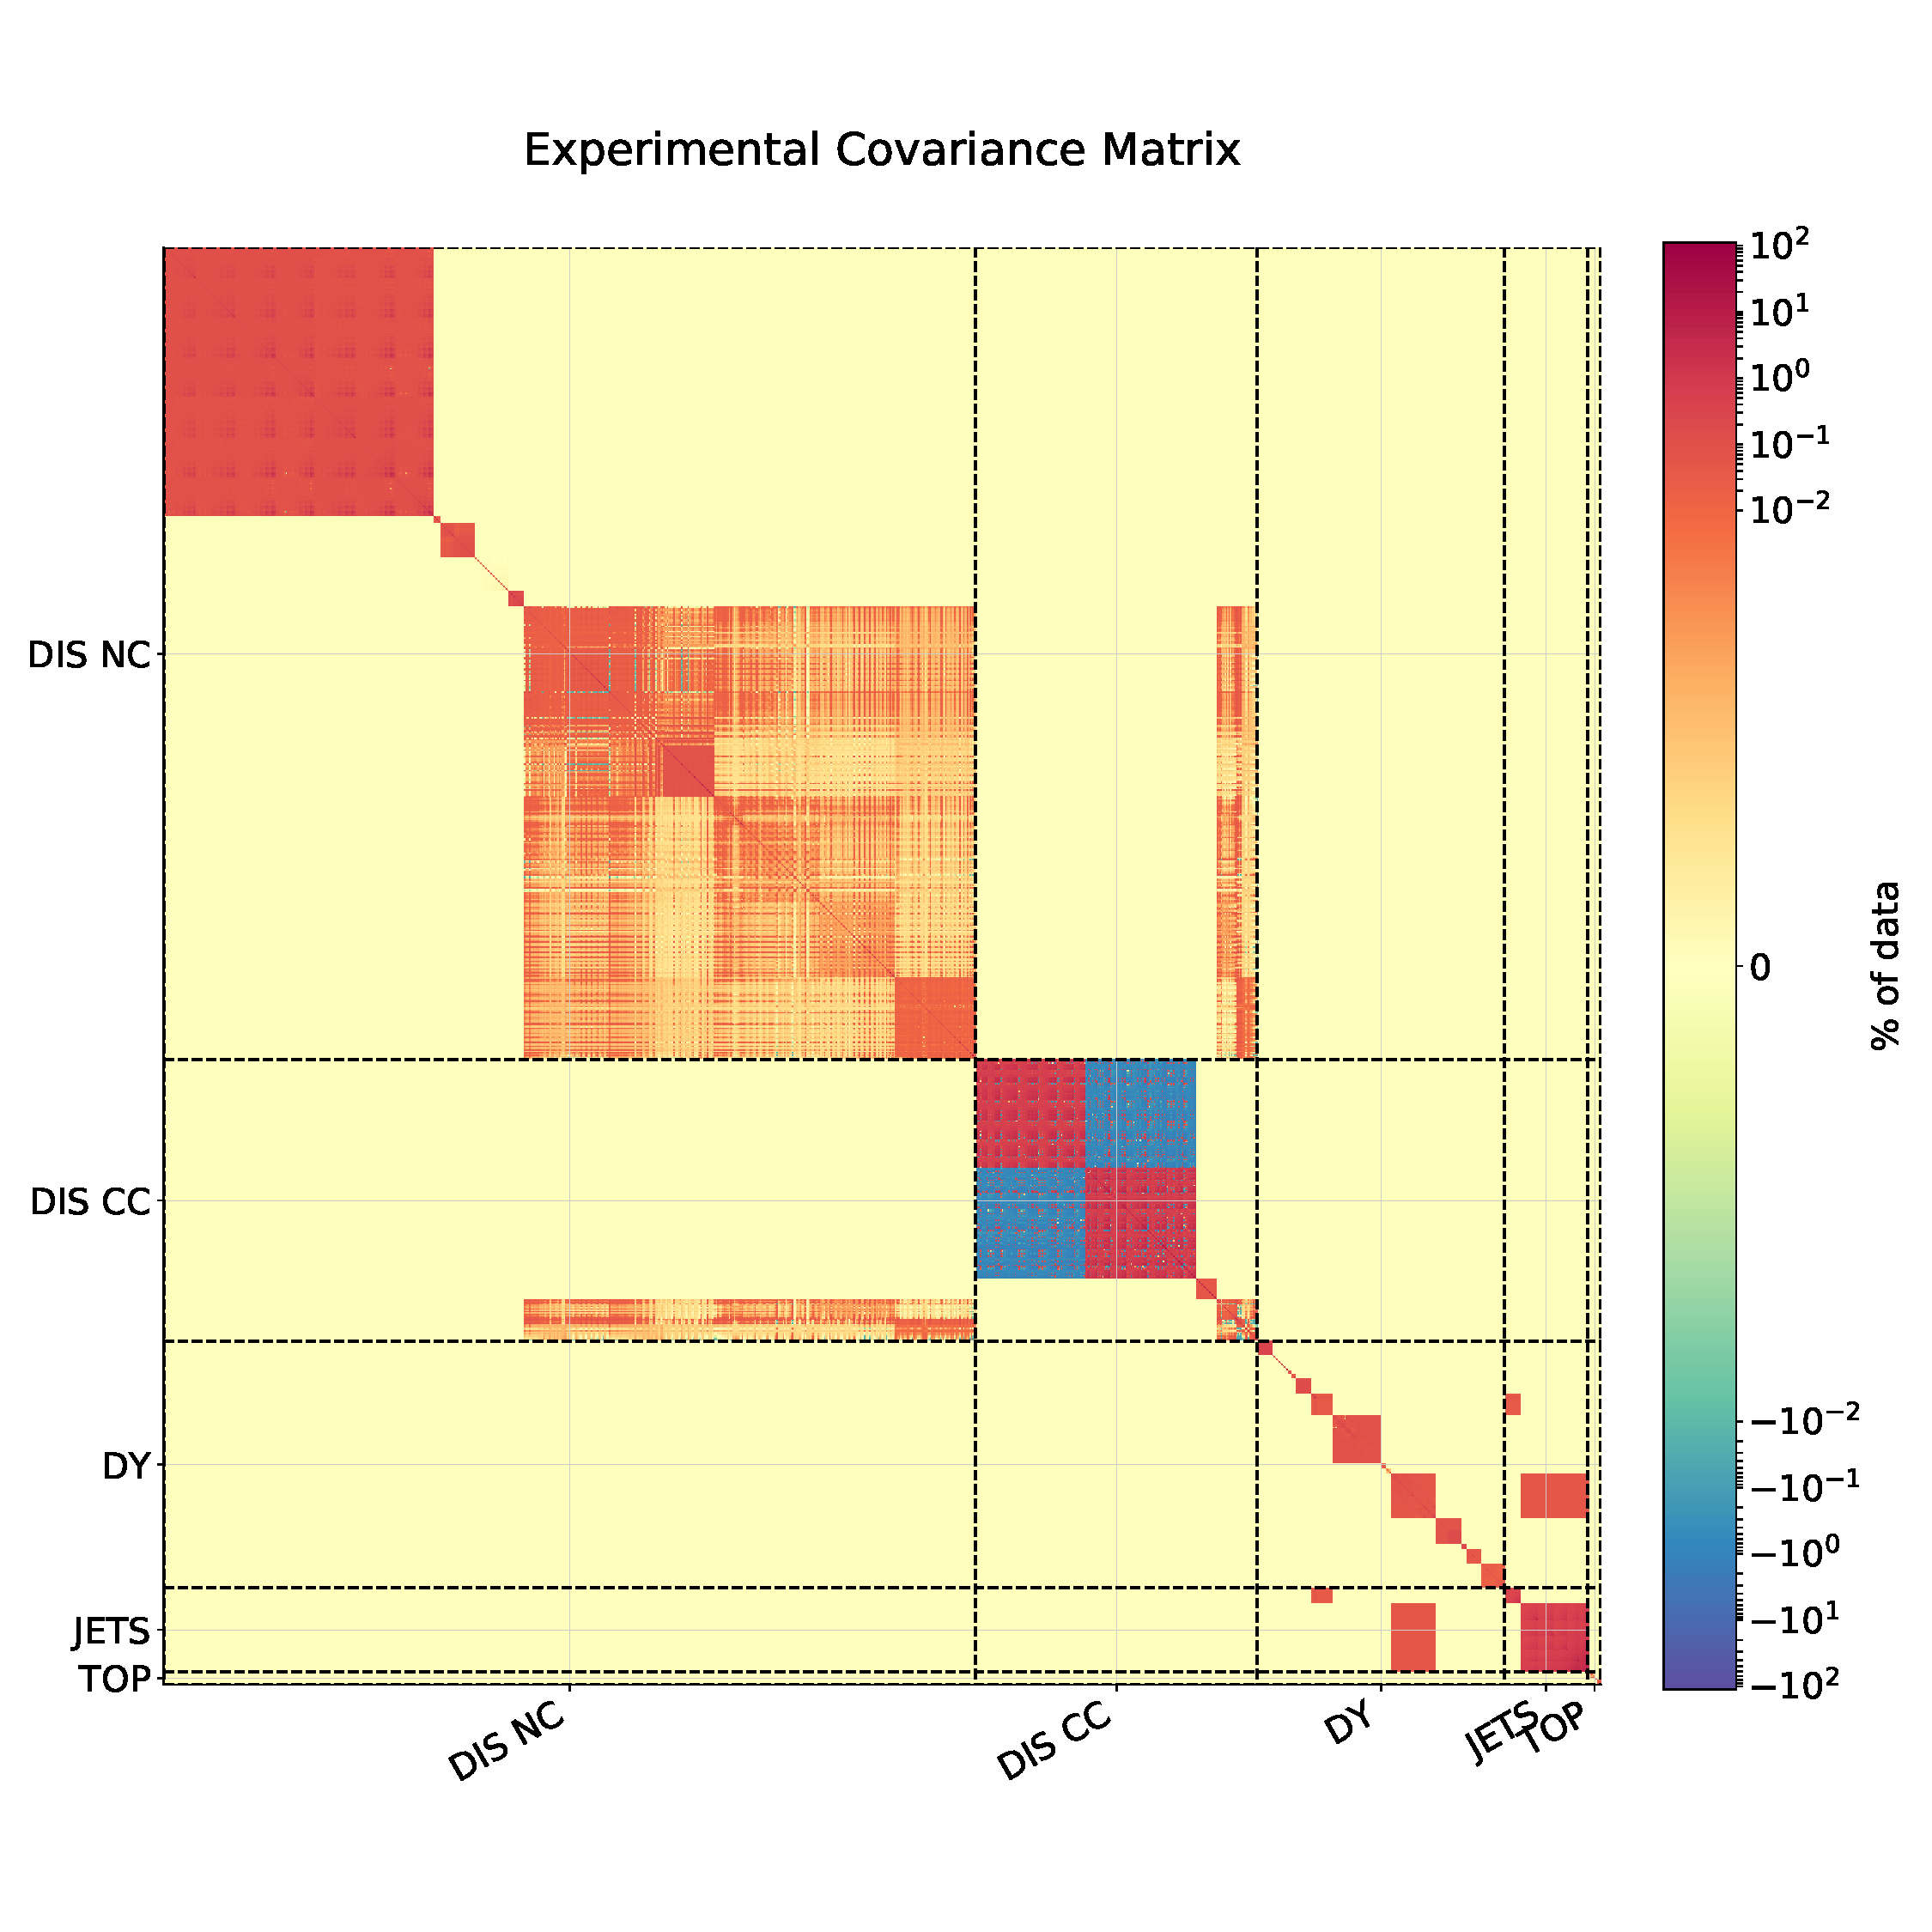
\includegraphics[width=0.49\linewidth]{exp_covmat.pdf}
        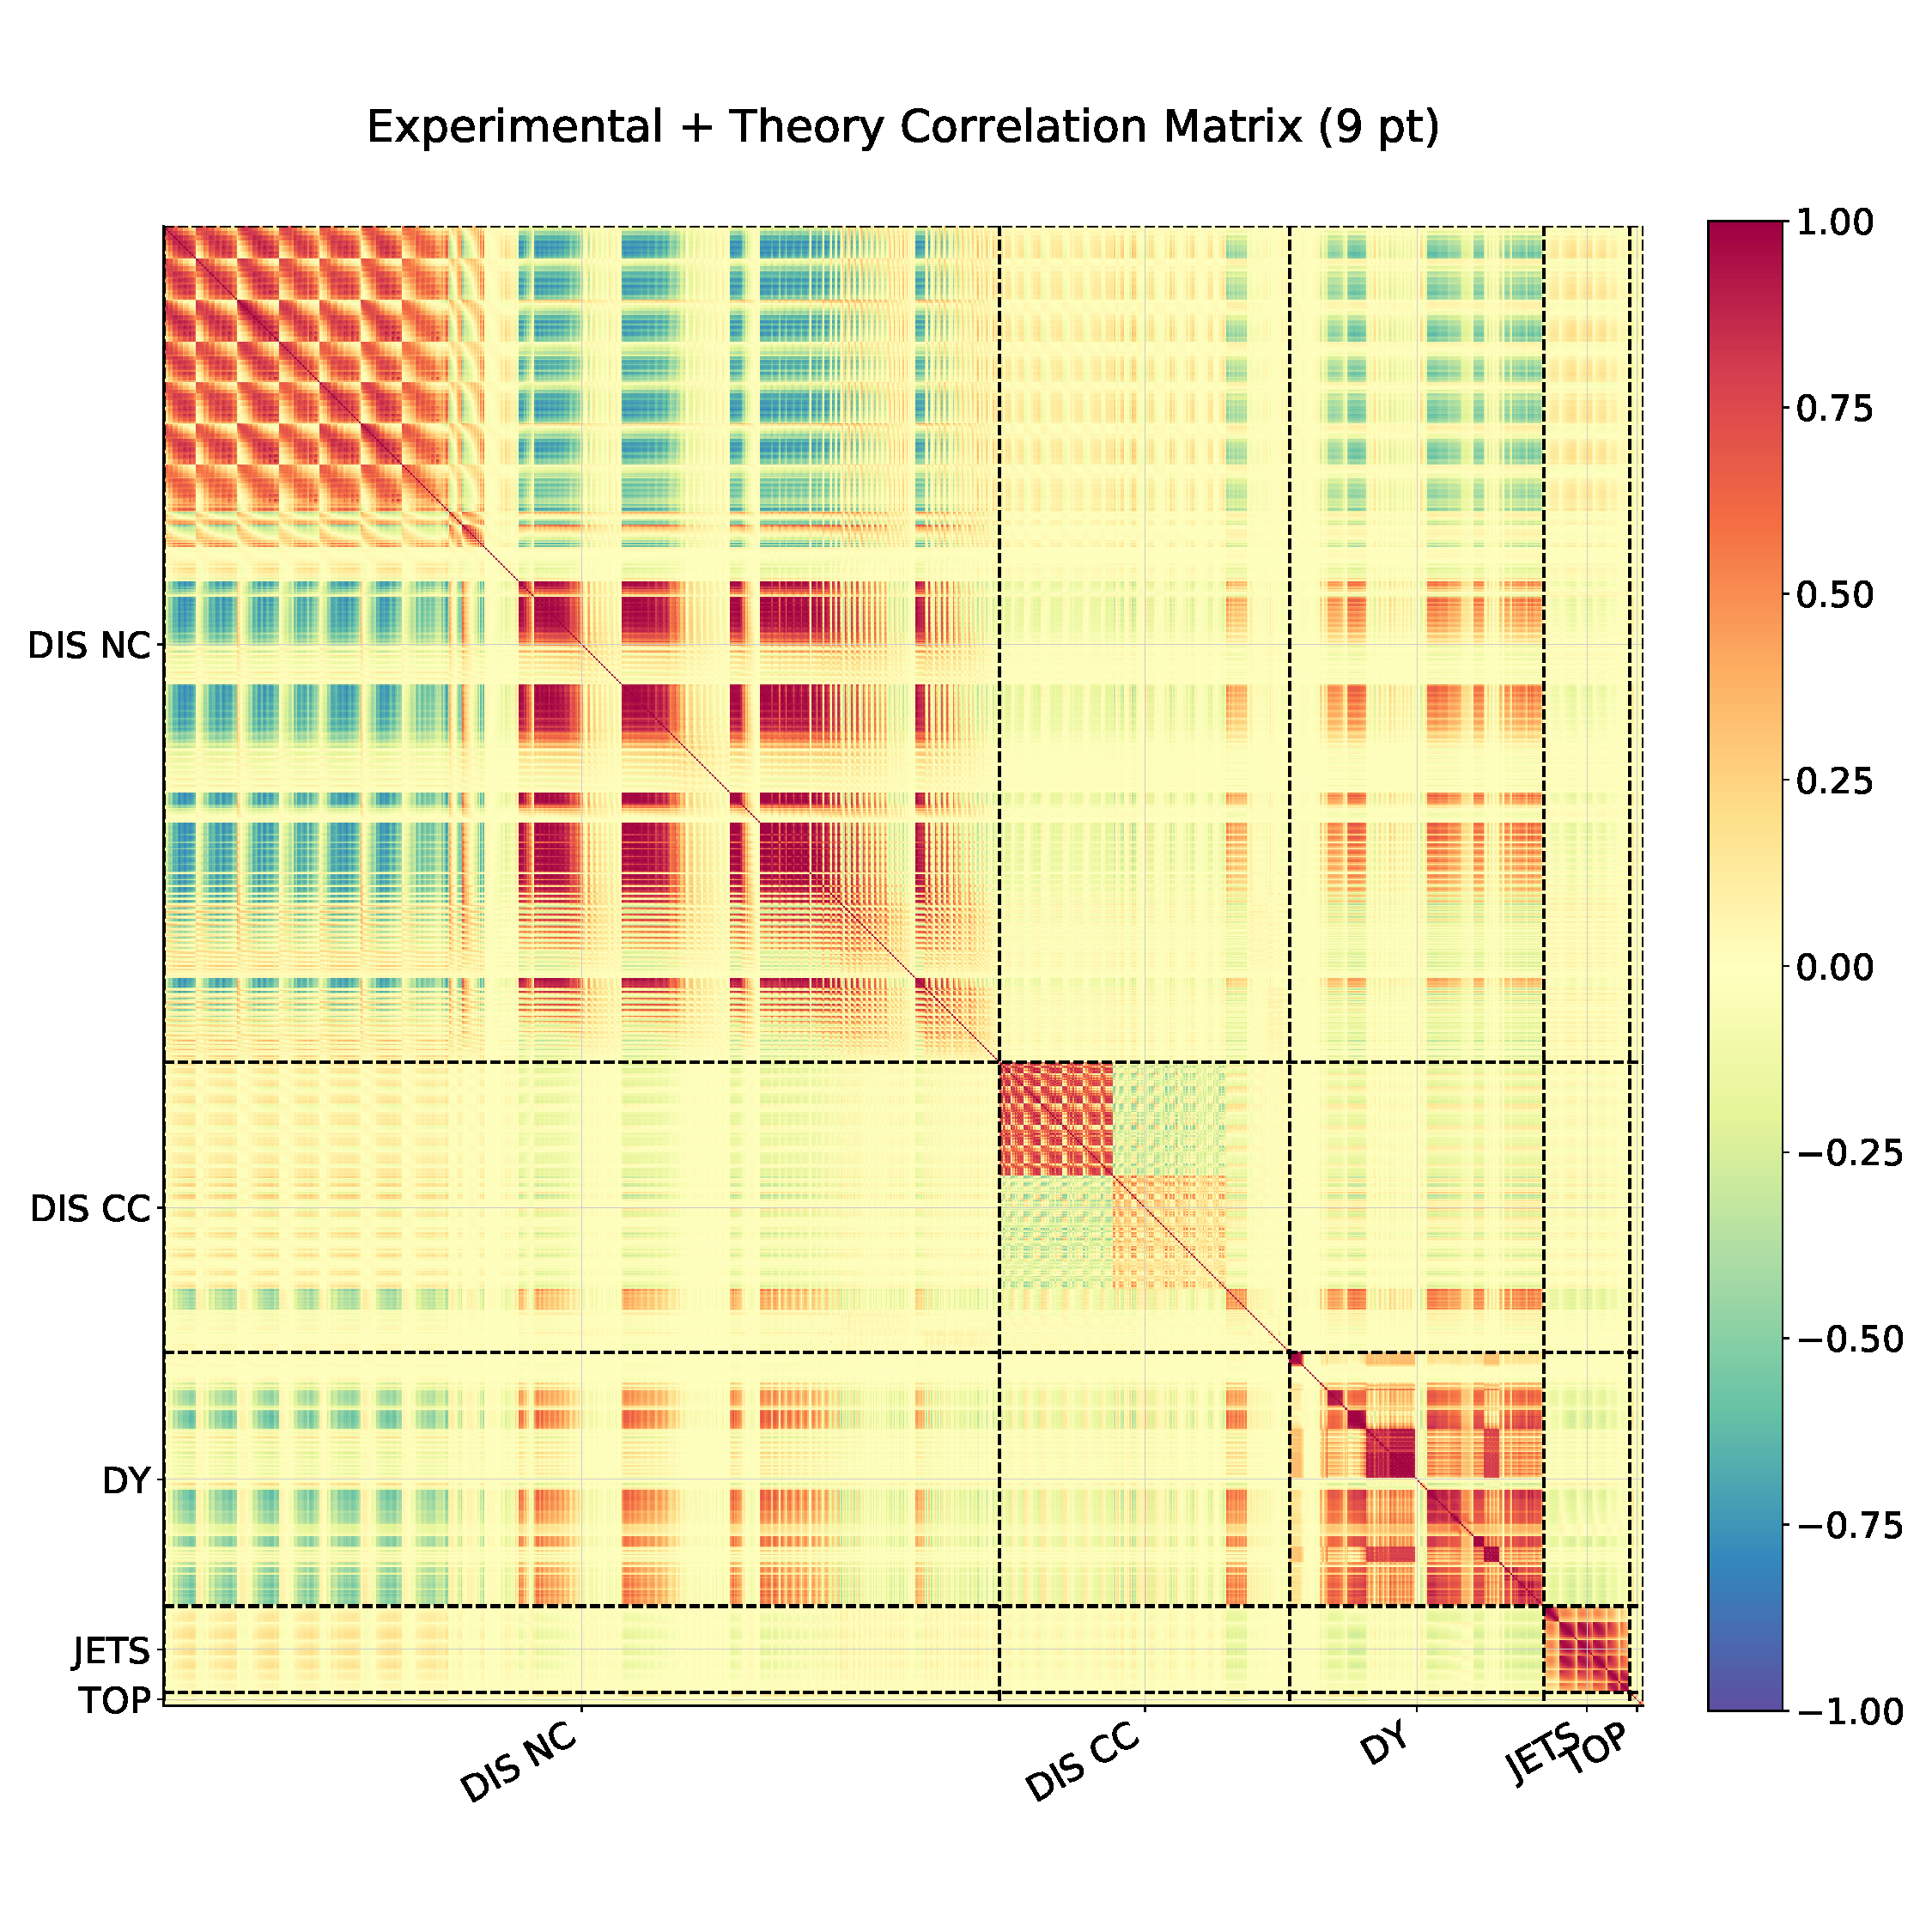
\includegraphics[width=0.49\linewidth]{expth_corrmat_9pt.pdf}
        \caption{\small Comparison of the  experimental $C_{ij}$ (left)
        and the combined experimental and theoretical correlation matrices $S_{ij}$, 
        All entries are normalized to the central  experimental value.
        The data are grouped by process and, within a process, by experiment. Figure from Ref.~\cite{AbdulKhalek:2019ihb}.} 
        \label{fig:covmats}     
    \end{center}
    \end{figure}

    %
    Next, we wish to construct a validation test for the NLO theory covariance matrix, using the known shift between
    NNLO and NLO results.
    In order to do this, we view the set of experimental data as a vector $D_i$, where $i = 1, ..., N_{dat}$.
    Such vector lives in a vector space $D$ of dimension $N_{dat}$, and
    the theory covariance matrix $S_{ij}$ defines an ellipsoid $E$ belonging to a subspace $S$ of dimension
    $N_{sub}$ of the full space $D$. 
    %
    In the context of MHOU we can take the NLO theory predictions evaluated at the central scales $T_i^{NLO}\left(0,0\right)$
    as our best NLO predictions with the ellipsoid $E$ estimating a $68\%$ confidence level for the MHO corrections. 
    We want to check how well the theory covariance matrix $S_{ij}$ predicts both the size and the correlation pattern
    of the MHO terms. This can be done by testing the extend by which the known shift vector between NNLO and NLO theory predictions
    $T_i^{NNLO} - T_i^{NLO}$
    falls within the ellipsoid $E$.
    %
    More in detail, we first normalize the theory covariance matrix $S_{ij}$ to the NLO predictions, so that all its
    entries are dimensionless allowing for a meaningful comparison 
    \begin{align}
        \hat{S}_{ij} = S_{ij}/\left(T_i^{NLO}T_j^{NLO}\right)\,,
    \end{align}
    and likewise we define a normalized shift vector as
    \begin{align}
        \delta_i = \left(T_i^{NNLO}-T_i^{NLO}\right)/T_i^{NLO}\,.
    \end{align}
    The NNLO predictions used to define the shift $\delta_i$ are computed using the NNLO matrix elements and anomalous dimensions
    but the same NLO PDF set used to compute the NLO theory predictions. In this way the shift $\delta_i$ 
    only accounts for the perturbative effects due to NNLO corrections, without including additional effects
    due to refitting.
    A first test to check whether the overall size of the scale variation is of the right order of magnitude
    consists into comparing the diagonal entries $\hat{S}_{ii} = \sigma_i^2$ to the normalized shift $\delta_i$.
    This check is performed in Fig.~\ref{fig:diag_shift_validation_symmetric}: in all cases 
    $\delta_i$ turns out to be smaller or comparable to $\sigma_i$, showing how how
    the overall size of the estimated uncertainties, obtained by varying the renormalization and factorization scales by
    a factor two in either directions, gives a qualitative reliable (if somewhat conservative) estimate of the true MHOU. 
    \begin{figure}[t!]
        \begin{center}
          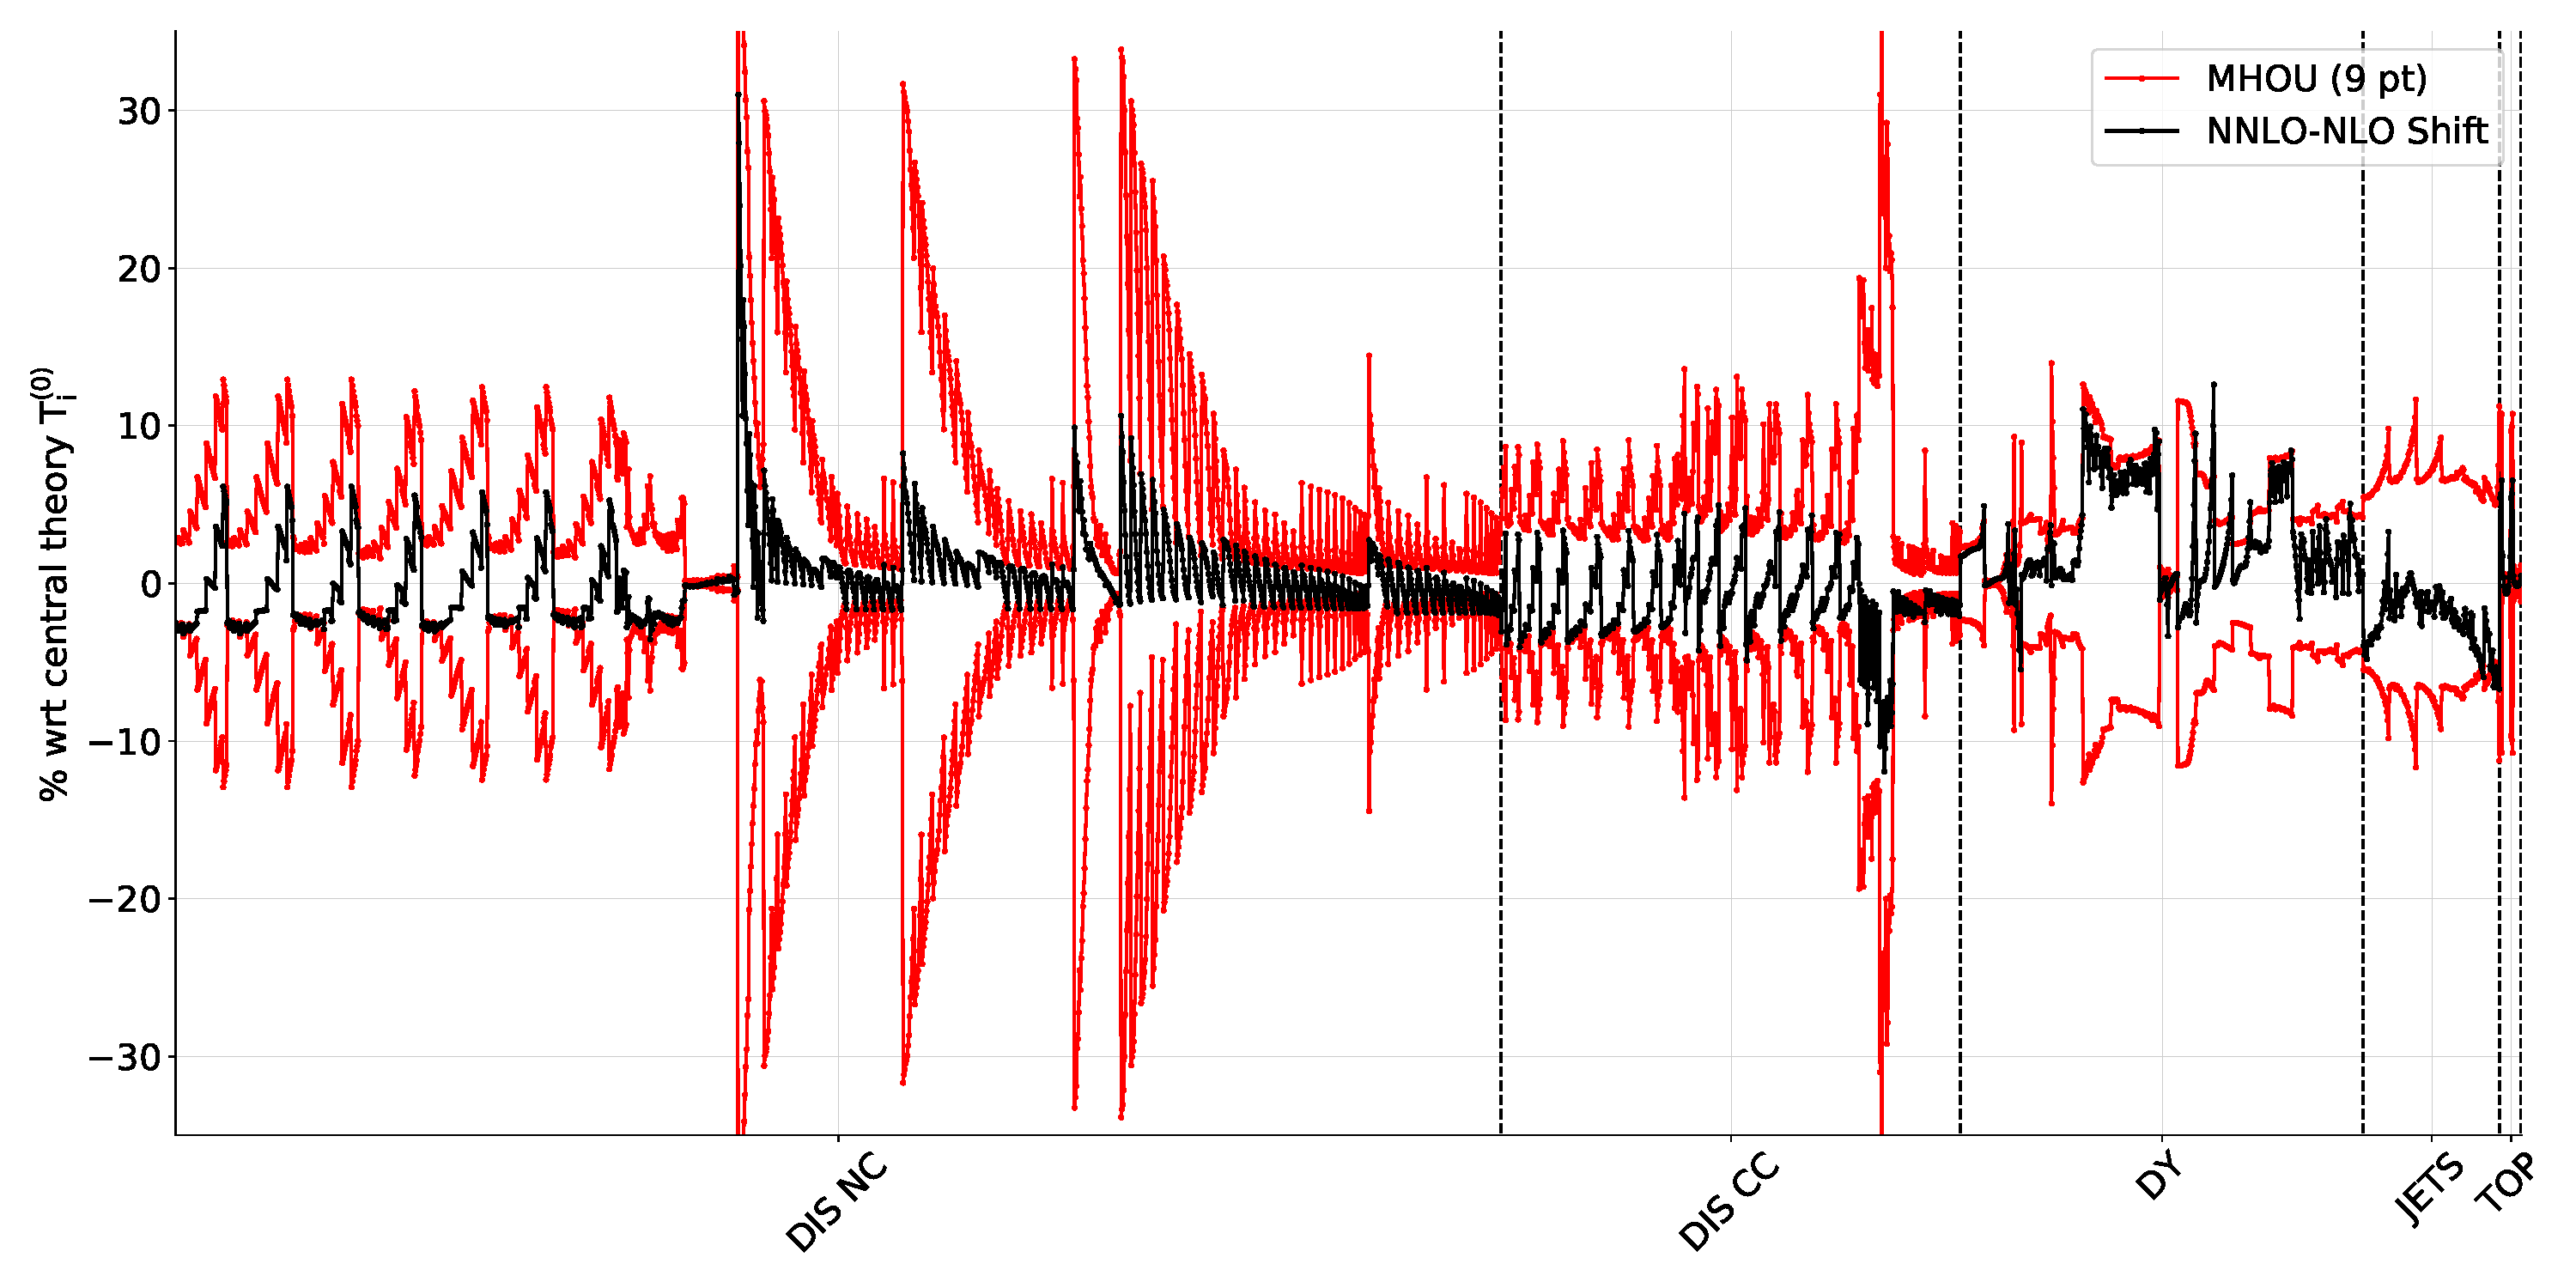
\includegraphics[width=14cm, height=4.4cm]{shift_diag_cov_comparison_9pt_global.pdf}
          \caption{\small The diagonal uncertainties  $\sigma_i$ (red)
            symmetrized about zero,
            compared to the shift $\delta_i$ (black) for each
            datapoint. Figure from Ref.~\cite{AbdulKhalek:2019ihb}.}
          \label{fig:diag_shift_validation_symmetric}
        \end{center}
    \end{figure}

    The validation of the full covariance matrix $\hat{S}_{ij}$ requires some more work.
    In order to identify the subspace $S$ we diagonalize the matrix $\hat{S}_{ij}$, getting a set
    of orthonormal eigenvectors $e_i^{\alpha}$ and the corresponding non-zero eigenvalues 
    $\lambda_{\alpha}$ with $\alpha = 1, ..., N_{sub}$.
    There is also a set of $N_{dat}-N_{sub}$ zero eigenvalues, corresponding to eigenvectors spanning
    the space $D/S$.
    In general the shift vector $\delta$ will live in the space $D$. 
    For a successful test we expect most of $\delta$ to lie within $S$.
    In other words, denoting as $\delta^s$ the projection of the shift over the subspace $S$
    \begin{align}
        \delta_i^s = \sum_{\alpha=1,...,N_{sub}} \delta^{\alpha}e^{\alpha}_i\,,
    \end{align} 
    we expect the angle $\theta$ between $\delta$ and $\delta^s$
    \begin{align}
        \label{eq:angle}
        \theta = \arccos\left(\frac{|\delta^s|}{|\delta|}\right)
    \end{align}
    to be reasonably small. This geometric relation is represented graphically in Fig.~\ref{fig:subspace_diagram},
    where the space $D$ is drawn as a three dimensional space and the subspace $S$ as a two dimensional space.
    For individual processes we find 
    \[\theta = 3^{\rm o}, 14^{\rm o}, 22^{\rm o}, 32^{\rm o}, 16^{\rm o}\]
    for top, jets, DY, NC and CC DIS respectively, 
    while for the complete dataset we find $\theta = 26^{\rm o}$.
    %
    \begin{figure}[t]
        \begin{center}
          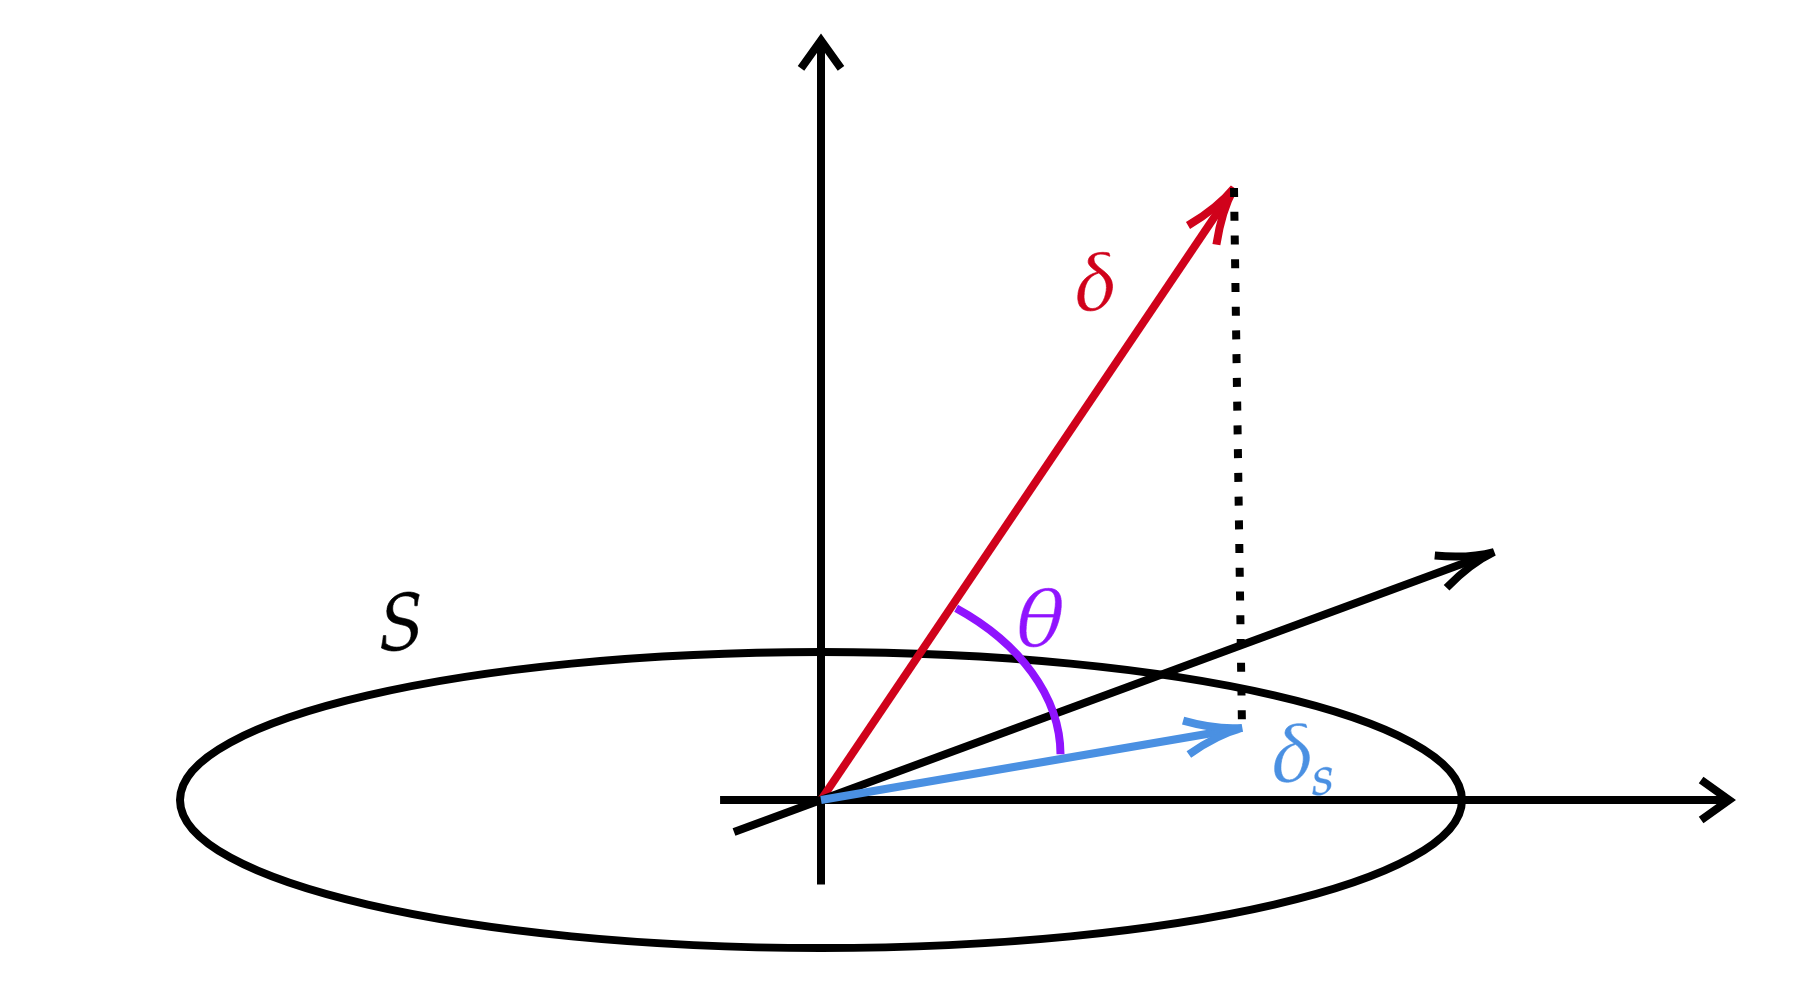
\includegraphics[scale=0.12]{subspace_diag.png}
          \caption{\small Schematic representation of the geometric relation
            between the shift vector $\delta\in D$ (here drawn as a three dimensional space), and
            the component $\delta^S$ of the shift vector which lies in the 
      subspace $S$ (here drawn as a two dimensional space, containing the ellipse E defined by the theory covariance matrix). 
      The angle $\theta$ between $\delta$ and $\delta^S$ is also shown. Figure from Ref.~\cite{AbdulKhalek:2019ihb}.
          \label{fig:subspace_diagram} }
        \end{center}
      \end{figure}
    %
    It is clear from these numbers how processes with larger numbers of data points, having 
    a wider kinematic range and thus more structure to predict, are much harder to describe than those 
    with only few data, which translates into bigger values of $\theta$ for bigger datasets. However in general the
    $\theta$ values we get for each specific process and for the global dataset result reasonably small, validating our definition
    and construction of a NLO theory covariance matrix.

    
    \section{NLO PDFs with missing higher order uncertainties}
    \label{sec:th_error_results}
    In this section we present the first determination of the proton PDFs 
    which systematically account for MHOU,
    using the theory covariance matrix formalism described in the previous sections.
    %
    We will present only a NLO fit, leaving a full NNLO analysis for a future work.
    Note that a NLO PDFs fit offers a nontrivial validation of our methodology, by comparing the results with and without MHOU to 
    a standard NNLO PDF set (obtained starting from the same input datasets).

    %
    As discussed in Sec.~\ref{sec:th_err_as_cov}, the theory uncertainties are included by replacing the
    experimental covariance matrix $C_{ij}$ with the sum $C_{ij}+S_{ij}$. The NNPDF methodology 
    described in chapter~\ref{ch:nnpdf_methodology} is otherwise unchanged.
    It is then clear how the inclusion of a theory-induced contribution in the covariance matrix affects only two steps
    of the fit: the pseudodata generation and the definition of the $\chi^2$ to be minimized.
    In particular, denoting as $D_i^{(k)}$ the $k$-th replicas for the $i$-th datapoint entering the analysis,
    we will now have
    \begin{align}
        \lim_{N_{rep}\rightarrow \infty}\frac{1}{N_{rep}-1}
        \sum_{k=1}^{N_{rep}}\left(D_i^{(k)}-\langle D_i \rangle\right)\left(D_j^{(k)}-\langle D_j \rangle\right)
        = C_{ij} + S_{ij}\,,
    \end{align}
    with $\langle D_i \rangle$ denoting the average over the $N_{rep}$ Monte Carlo pseudodata.
    Each PDF replica is then fitted by minimizing 
    \begin{align}
        \chi^2 = \frac{1}{N_{dat}}\sum_{i,j=1}^{N_{dat}}
        \left(D_i - T_i\right)\left(C+S\right)_{ij}^{-1}\left(D_j-T_j\right)\,,
    \end{align}
    where the theory predictions $T_i$ are computed using the central scales choice.
    %
    In the following, in order to asses the fit quality and to study the impact of MHOUs on the final
    PDF uncertainties, we will provide values for the total and partial $\chi^2$ and for the estimator
    $\phi$, defined in Ref.~\cite{Ball:2014uwa} as
    \begin{align}
        \label{eq:phi}
        \phi = \sqrt{\langle \chi^2_{\text{exp}}\left[T^{(k)}\right] \rangle 
        - \chi^2_{\text{exp}}\left[\langle T^{(k)} \rangle\right]}\,,
    \end{align}
    where by $\chi^2_{\text{exp}}\left[T^{(k)}\right]$ we denote the value of the $\chi^2$
    computed using the $k$-th PDF replica and only including the experimental covariance matrix.
    The average $\chi^2$ values entering Eq.~\eqref{eq:phi} are the $\chi^2$ averaged over the replicas
    and the $\chi^2$ computed using the central PDF, which is obtained as an average of all replicas. 
    As shown in App.~\ref{app:phi} Eq.~\eqref{eq:phi} can be written as
    \begin{align}
        \phi = \left(\frac{1}{N_{dat}}\sum_{i,j=1}^{N_{dat}} \left(C\right)^{-1}_{ij}T_{ij}\right)^{1/2}\,,
    \end{align}
    where $T_{ij} = \langle T^{(k)}_i T^{(k)}_j \rangle - \langle T^{(k)}_i \rangle \langle T^{(k)}_j \rangle$. In words,
    $\phi$ gives the average over all the datapoints of the ratio of the uncertainties of the predictions
    to the uncertainties of the original experimental data, taking correlations into account. For a purely diagonal
    covariance matrix, this would be the ratio of the uncertainty of the predictions using the output PDFs
    to that of the original data. Note that  $\phi$ is defined in such a way that the uncertainty in the prediction is always
    normalized to the experimental uncertainty, rather then to the combined experimental and theoretical uncertainty.
    By comparing $\phi$ values for fits with and without MHOU we can then get a quantitative idea of the effect of theory
    uncertainty on the final PDF error.

    %
    In order to asses the effect of MHOU, in addition to fits with the theory covariance matrix, two baseline
    NLO and NNLO fits based on the experimental covariance matrix $C$ only have been also produced, 
    using the same input datasets described in Section ~\ref{sec:validation}. 
    As mentioned previously, including a new contribution to the covariance matrix of the fit
    will affect both the PDFs central value of and uncertainty. In order to disentangle these
    two different effects, we also study PDFs determined by only partially 
    including the theory covariance matrix $S$ in the analysis, either only in the data generation or in the fitting. 
    %
    The PDF sets which will be discussed in the following are reported in Table ~\ref{tab:thcovmatFits}. 
    For each fit we indicate its labels, the perturbative order and the covariance matrix used.
    %%%%%%%%%%%%%%%%%%%%%%%%%%%%%%%%%%%%%%%%%%%%%%%%%%%%%%%%%%%%%%%%%%%%%%%%%%%
%%%%%%%%%%%%%%%%%%%%%%%%%%%%%%%%%%%%%%%%%%%%%%%%%%%%%%%%%%%%%%%%%%%%%%%%%%%
\begin{table}[t]
  \centering
\footnotesize
  \renewcommand*{\arraystretch}{1.50}
  \begin{tabular}{lcccc}
    Label                    & $\quad$Order$\quad$  & Cov. Mat. &  Comments \\
    \toprule
        {\tt NNPDF31\_nlo\_as\_0118\_kF\_1\_kR\_1}  &      NLO  & $C$  & baseline Global NLO  \\
        {\tt NNPDF31\_nlo\_as\_0118\_scalecov\_9pt}  &     NLO  & $C+S$  &  \\
        \midrule
         {\tt NNPDF31\_nlo\_as\_0118\_scalecov\_9pt\_fit}  &     NLO  & $C+S$  & $S$ only in $\chi^2$
            definition \\
            {\tt NNPDF31\_nlo\_as\_0118\_scalecov\_9pt\_sampl}     &   NLO  & $C+S$  & $S$ only in sampling \\
            \midrule
        {\tt NNPDF31\_nnlo\_as\_0118\_kF\_1\_kR\_1}  &  Global     & $C$  & baseline Global NNLO  \\
            \bottomrule
  \end{tabular}
  \vspace{0.3cm}
  \caption{\small Summary of the PDF sets discussed in this
    section. The perturbative order and nature of the
    treatment of uncertainties for each set are indicated.
    \label{tab:thcovmatFits}
  }
  \end{table}
%%%%%%%%%%%%%%%%%%%%%%%%%%%%%%%%%%%%%%%%%%%%%%%%%%%%%%%%%%%%%%%%%%%%%%%%%%%%
%%%%%%%%%%%%%%%%%%%%%%%%%%%%%%%%%%%%%%%%%%%%%%%%%%%%%%%%%%%%%%%%%%%%%%%%%%%%    


    %
    The $\chi^2$ and $\phi$ values are shown in Tables ~\ref{table:chi2table_covth_global_nlo}
    and \ref{table:phitable_covth_global_nlo} respectively, for both the total dataset and the individual processes of 
    Table~\ref{eq:expclassification}.
    For all the processes, when including $S$ in the fit the $\chi^2$ decreases, improving
    by about $3\%$ when considering the total dataset. Additionally the total $\chi^2$ almost coincides with the NNLO 
    $\chi^2$, suggesting that indeed the theory uncertainty is correctly accounting for the missing NNLO corrections.
    Looking at the value of $\phi$, we notice how, interestingly, this only increases by around $30\%$, 
    much less than the $70\%$ one would expect looking at the relative size of the NLO MHOU and experimental uncertainties.
    These numbers suggest that the main effect of the inclusion of the theory covariance matrix is that
    in the data region tensions which are otherwise present in the global dataset due to the MHO are partially resolved,
    leading to a better fit quality without any major effect on the final PDFs error. 
    %
    Looking at the fits where the theory error is included in the $\chi^2$ but not in the replicas generation,
    it is clear how the inclusion of the theory covariance matrix in the 
    $\chi^2$ definition alone leads to a final $\chi^2$ value very close to that of the fit where the MHOU are fully included.
    This means that, as we would expect, the MHOU affect mostly the central value of the fit,
    since the relative weight carried by each point is altered during the fit according to their relative size of their MHOU.
    On the other hand, considering the case where the theory covariance matrix is included only in the replica generation, 
    the $\chi^2$ goes up and $\phi$ increases dramatically, pointing out a much more prominent effect in PDFs uncertainty.
    This behaviour is expected: due to the inclusions of MHOU in the pseudodata generation the replica fluctuations are wider,
    leading to an increase in the PDFs error, which is now uncompensated by a rebalancing of the datasets in the fits.
    %%%%%%%%%%%%%%%%%%%%%%%%%%%%%%%%%%%%%%%%%%%%%%%%%%%%%%%%%%%%%%%%%%%%%%%%%%%%%%%%%%%%%%%%%%%%%%%%%
\begin{table}[t]
\begin{center}
\renewcommand*{\arraystretch}{1.78}
\footnotesize
\begin{tabular}{|l|c|c|c|cc|c|}
  \toprule
  &    & \multicolumn{5}{c|}{$\chi^2/n_{\rm dat}$ in the NNPDF3.1 global fits}   \\
 Process & $n_{\rm dat}$ & \multicolumn{4}{c|}{NLO}  & NNLO  \\
 &  & $C$ & $C+S^{(\rm 9pt)}$   &   $C+S^{(\rm 9pt)}_{\rm fit}$ &
  $C+S^{(\rm 9pt)}_{\rm sampl}$   &  $C$ \\
\toprule
DIS NC    & 1593 & 1.088  & 1.079   &  1.081 & 1.227 & 1.084 \\
DIS CC    & 552  & 1.012  & 0.928   &  0.929 & 1.036 & 1.079 \\
\midrule  
DY        & 484  & 1.486  & 1.447   &  1.461 & 1.434 & 1.231 \\
JETS      & 164  & 0.907  & 0.839   &  0.848 & 0.911 & 0.950 \\
TOP       & 26   & 1.260  & 1.012   &  1.001 & 1.264 & 1.068 \\
\midrule
Total     & 2819 & 1.139  & 1.109   &  1.113 & 1.217 & 1.105 \\
\bottomrule
\end{tabular}
\end{center}
\caption{The values of the $\chi^2/N_{\rm dat}$ 
  in the NNPDF3.1 global fits with the theory covariance matrix $S$, compared to the results based on including only
  the experimental covariance matrix $C$. We also show  results obtained
  including the theory covariance matrix only in the $\chi^2$ definition but not
  in the data generation and conversely.
  Values corresponding to the NNLO fit with  experimental covariance matrix $C$ only are also shown.
  \label{table:chi2table_covth_global_nlo}
}
  \end{table}
%%%%%%%%%%%%%%%%%%%%%%%%%%%%%%%%%%%%%%%%%%%%%%%%%%%%%%%%%%%%%%%%%%%%%%%%%%%%%%%%%%%%%%%%%%%%%%%%%
  
    %%%%%%%%%%%%%%%%%%%%%%%%%%%%%%%%%%%%%%%%%%%%%%%%%%%%%%%%%%%%%%%%%%%%%%%%%%%%%%%%%%%%%%%%%%%%%%%%%
\begin{table}[t]
\begin{center}
\renewcommand*{\arraystretch}{1.78}
\footnotesize
\begin{tabular}{|l|c|c|cc|c|}
  \toprule
  & \multicolumn{5}{c|}{$\phi$ in the NNPDF3.1 global fits}   \\
 Process & \multicolumn{4}{c|}{NLO}  & NNLO  \\
 & $C$ & $C+S^{(\rm 9pt)}$   &  $C+S^{(\rm 9pt)}_{\rm fit}$ &
  $C+S^{(\rm 9pt)}_{\rm sampl}$   &  $C$ \\
  \toprule
  DIS NC     & 0.266 & 0.412 &  0.414 & 1.137 & 0.305 \\
  DIS CC     & 0.389 & 0.408 &  0.388 & 0.502 & 0.471 \\
  \midrule
  DY         & 0.361 & 0.377 &  0.378 & 0.603 & 0.380 \\
  JETS       & 0.295 & 0.359 &  0.336 & 0.461 & 0.392 \\
  TOP        & 0.375 & 0.443 &  0.382 & 0.612 & 0.363 \\
  \midrule
  Total      & 0.314 & 0.405 &  0.400 & 0.932 & 0.362 \\
  \bottomrule
\end{tabular}
\end{center}
\caption{Same as Table~\ref{table:chi2table_covth_global_nlo}, but 
  for the values of the $\phi$ estimator.
  \label{table:phitable_covth_global_nlo}}
  \end{table}
%%%%%%%%%%%%%%%%%%%%%%%%%%%%%%%%%%%%%%%%%%%%%%%%%%%%%%%%%%%%%%%%%%%%%%%%%%%%%%%%%%%%%%%%%%%%%%%%%
 
    
    %
    In Fig.~\ref{fig:pdfs_plots_th_err} we show plots for the NLO PDFs of the gluon, the total quark singlet,
    the anti-down quark and the strange, comparing results for fits based on $C$ and $C+S$.
    All the PDFs are plotted at $Q=10$ GeV and normalized to the fit results without MHOU, 
    and the central value of the NNLO fit based on the experimental covariance matrix only is shown as well.
    %
    We find that in the data region the increase in PDF uncertainties is very moderate, while the central values 
    can shift by up to one sigma. On the other hand, in the regions where the PDFs are loosely constrained by the experimental
    data the PDF uncertainties increases significantly.
    These features are in agreement with the observation that the estimator $\phi$, whose values are reported 
    in Table~\ref{table:phitable_covth_global_nlo}, increases only by a moderate amount when including the theory error,
    and provide further evidence that in the data region the inclusion of the theory covariance matrix has resolved tensions
    due to MHO.
    % 
    This point can be further supported by observing the improvement in the agreement between the best-NLO fit and the NNLO PDFs
    (the latter with experimental covariance matrix only): looking at the central value of the NNLO fit, 
    first it is fully compatible with the uncertainty band of the NLO fit, second it is evident how upon inclusion of 
    the NLO MHOU the central best fit moves towards the correct NNLO result.
    This is particularly evident in the case of the gluon and of the strangeness, where inclusion of MHOU leads to a
    suppression at large $x$ of the first and to an enhancement in the whole $x$ region of the second.  
    \begin{figure}[t!]
        \begin{center}
            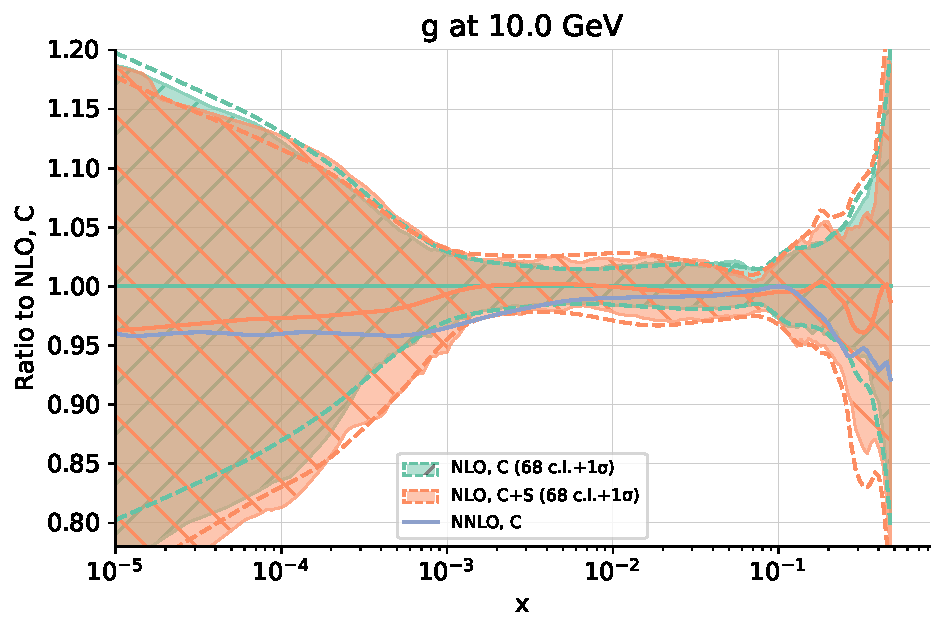
\includegraphics[width=0.49\linewidth]{plot_pdfs_g.pdf}
            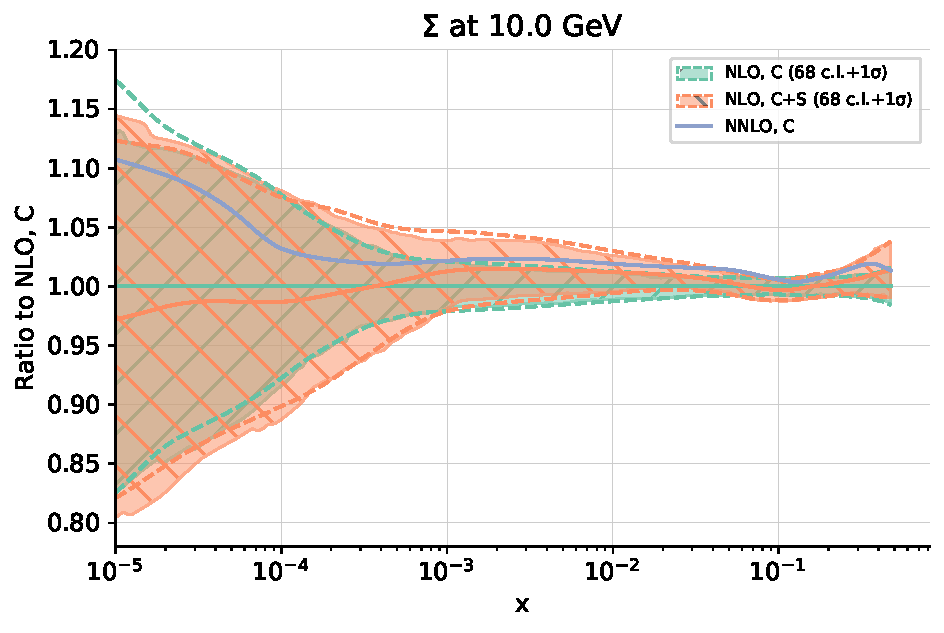
\includegraphics[width=0.49\linewidth]{plot_pdfs_Sigma.pdf}
            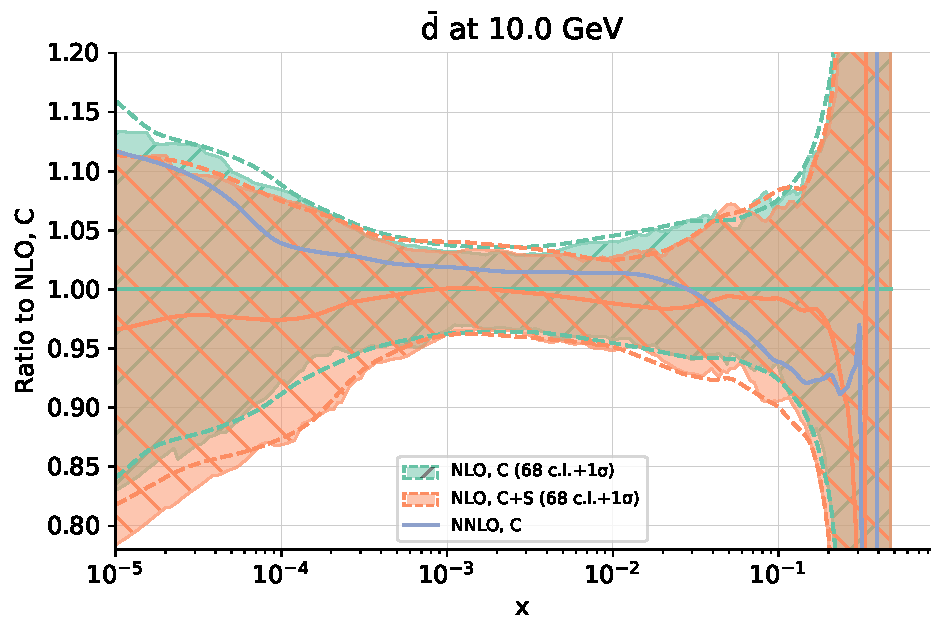
\includegraphics[width=0.49\linewidth]{plot_pdfs_bard.pdf}
            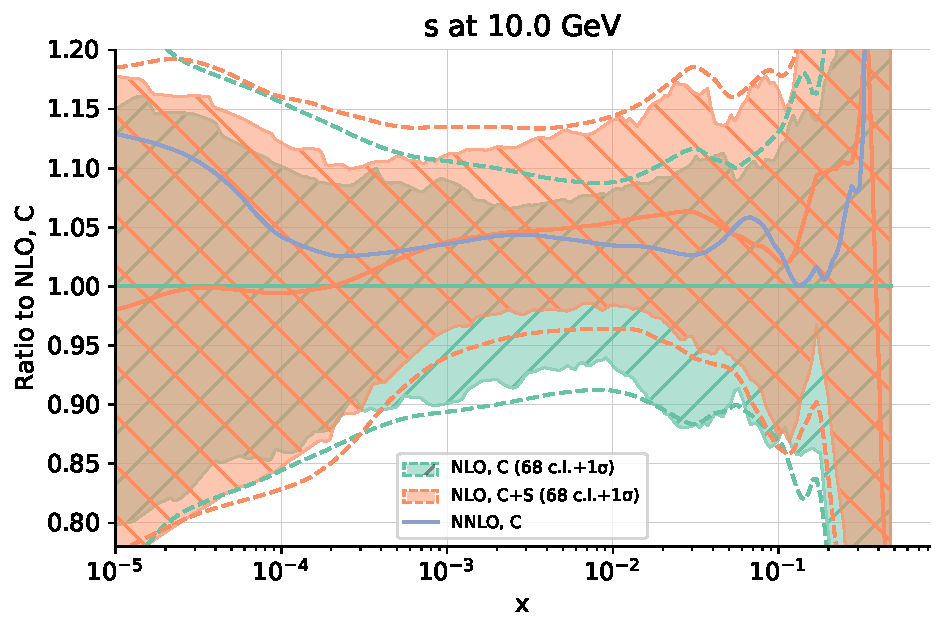
\includegraphics[width=0.49\linewidth]{plot_pdfs_s.pdf}
            \caption{Results of the NLO fits based on $C$ and $C + S$ normalized to the
            former, as well as the central value of the NNLO fit based on $C$ for the gluon, the total quark singlet, 
            the anti-down quark, and the strange PDFs, all at $Q = 10$ GeV.} 
            \label{fig:pdfs_plots_th_err} 
        \end{center}
    \end{figure}

    %
    Finally in Fig.~\ref{fig:pdfs_plots_th_err_mc_chi2} we look at PDFs where the theory covariance matrix has been
    included in the $\chi^2$ definition but not in the Monte Carlo replicas generation and conversely.
    It is clear from the plots how, when $S$ is included in the data replica generation only, 
    uncertainties increased significantly. This is in agreement with the numbers observed in 
    Tables~\ref{table:chi2table_covth_global_nlo} and \ref{table:phitable_covth_global_nlo}: the wider fluctuations 
    in the data generation are not matched by the $\chi^2$ definition, resulting in an overall bigger error and a worse
    fit quality.
    On the other hand, when $S$ is included only in the $\chi^2$ definition, the effect of theory error on
    the central value of the fit is singled out: the central value of the fit is very close to that obtained 
    when including the MHOU in both data generation and fit, and, consistently with Table~\ref{table:phitable_covth_global_nlo},
    the change of the PDFs error in the data region is very small.
    This confirms our previous statement according to which, while the addition of a theory covariance matrix
    in replicas generation increases the fluctuations of the data replicas, this is compensated by the inclusion of MHOU
    in the fit, which releases tensions between dataset, with the net results that, while the central values shift, 
    the uncertainties in the data region do not increase much.
    \begin{figure}[t!]
        \begin{center}
            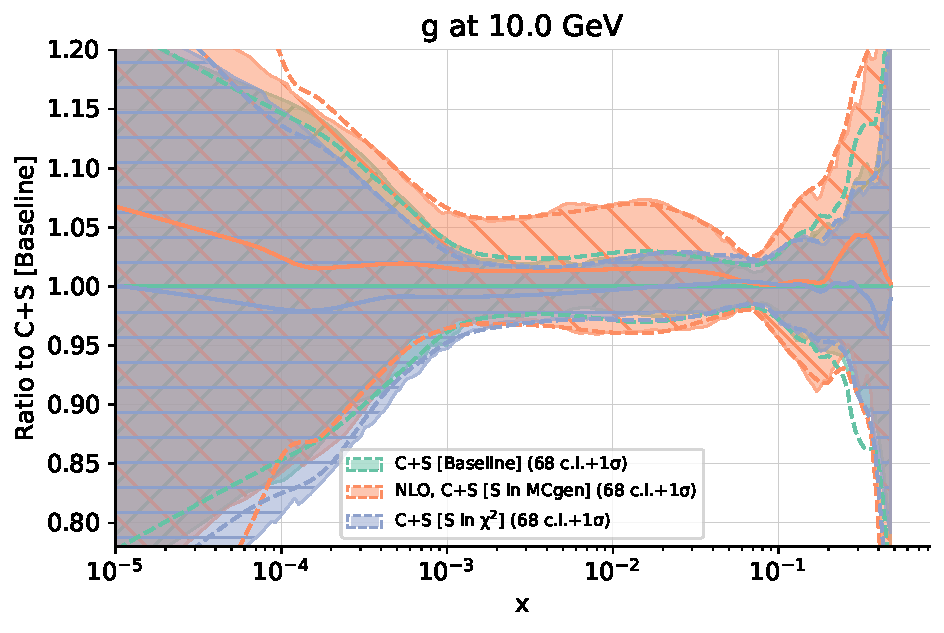
\includegraphics[width=0.49\linewidth]{plot_pdfs_g_mc_chi2.pdf}
            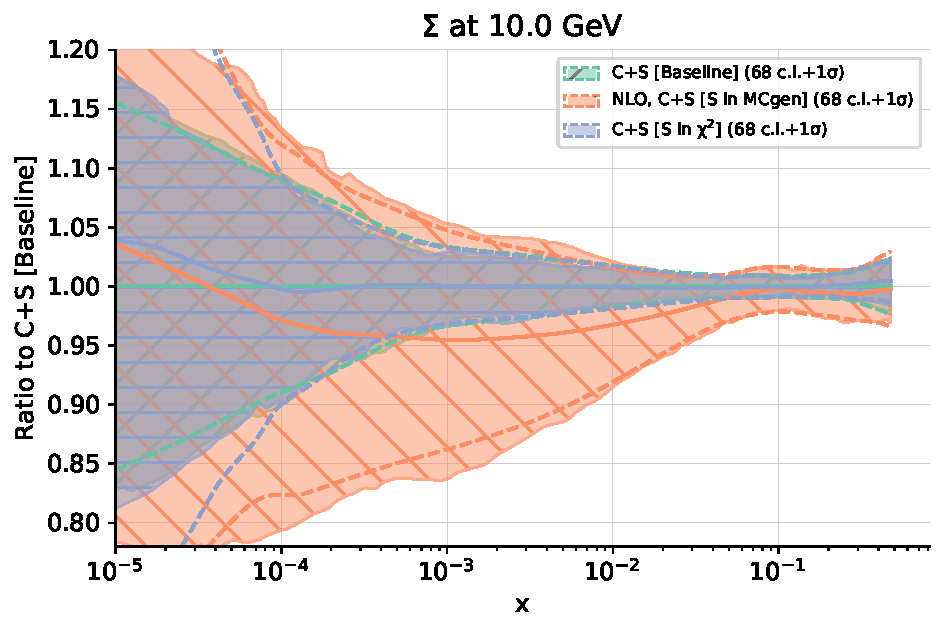
\includegraphics[width=0.49\linewidth]{plot_pdfs_Sigma_mc_chi2.pdf}
            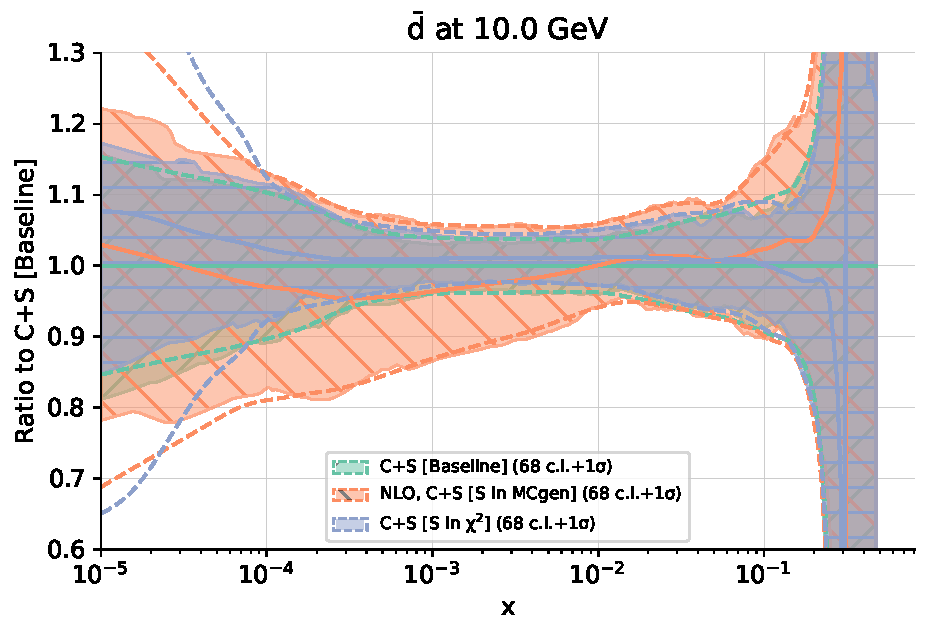
\includegraphics[width=0.49\linewidth]{plot_pdfs_bard_mc_chi2.pdf}
            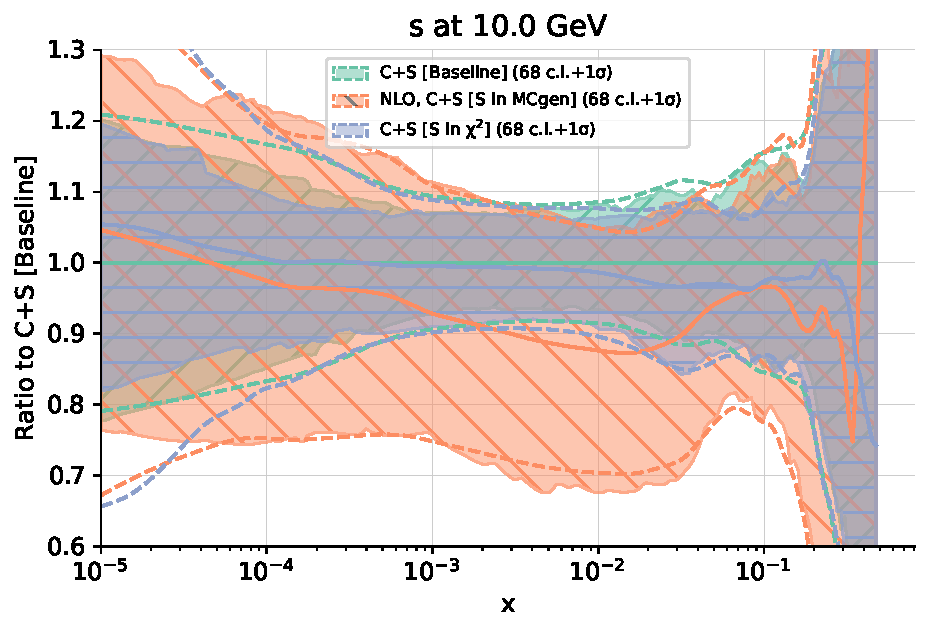
\includegraphics[width=0.49\linewidth]{plot_pdfs_s_mc_chi2.pdf}
            \caption{Same as Fig.~\ref{fig:pdfs_plots_th_err}, now comparing the results of the baseline $C + S$
            fit with those in which the theory covariance matrix $S$ is included
            either in the $\chi^2$ definition or in the generation of Monte Carlo replicas, but not in both} 
            \label{fig:pdfs_plots_th_err_mc_chi2} 
        \end{center}
    \end{figure}

    \section{Usage and delivery}
    \label{sec:th_error_usage}
    The PDFs with theory error can be used in the same way as a standard Monte Carlo PDF sets.
    In this section we briefly discuss how to combine the PDF theory error with that in that hard matrix elements,
    providing detailed instructions to use the results presented in Sec.~\ref{sec:th_error_results}. 

    %
    The MHOU on PDFs discussed here arise from the fact that the PDFs are determined using finite order
    perturbative computations: parton distributions obtained by using different perturbative orders in the computations
    for the input processes will be different (so that for example NLO PDFs differ from NNLO PDFs), and the formalism
    developed here provides a way to take this into account when working at some finite order in
    perturbation theory. 
    We have further seen how there exist two distinct sources of MHOU in PDFs, the first due to the computation
    of the hard cross-sections for partonic processes, the second due to the computation of the anomalous dimension.
    Considering a factorized prediction for some other process not used during the PDFs determination, 
    an additional source of MHOU is the computation of the hard process itself, which in turn will 
    carry MHOU related to the computation of the hard cross-section and MHOU related to the evolution of the PDF
    from the initial scale (at which the PDFs are delivered) to the scale of the process.
    In summary, each theory prediction for a factorized cross section carry two different MHOU,
    a PDFs uncertainty, discussed in this work, and an uncertainty arising in the calculation of the prediction itself. 
    We will ignore any possible correlation between these two different source of MHOU, 
    considering the two theory error as completely independent.
    
    %
    In the following we summarize our procedure to compute the total uncertainty for a given factorized
    cross-section $\mathcal{F}$.
    The PDF uncertainty $\sigma_{\mathcal{F}}^{\text{PDF}}$ can be evaluated in the same way as usually done
    for a standard Monte Carlo PDFs set, as the standard deviation over the replicas set
    \begin{align}
        \label{eq:PDFunc}
        \sigma_{\mathcal{F}}^{\text{PDF}} = 
        \left(\frac{1}{N_{\text{rep}}-1} \sum_{k=1}^{N_{\text{rep}}}
        \left(\mathcal{F}\left[\{q^{(k)}\}\right]-\langle \mathcal{F}\left[\{q\}\right] \rangle\right)^2
         \right)^{\frac{1}{2}}\,.
    \end{align}
    Considering the PDFs presented in this work, $\sigma_{\mathcal{F}}^{\text{PDF}}$ will account for
    uncertainties related to both experimental data and MHO in the PDFs determination.
    On the other hand, when Eq.~\eqref{eq:PDFunc} is used with a standard PDFs set (like NNPDF3.1), the resulting
    uncertainty only incudes statistical and systematic errors from the data. 
    Turning to MHOU on the hard matrix element $\sigma_{\mathcal{F}}^{\text{th}}$,
    this can be estimated using any prescription preferred by the user.
    A commonly used procedure is given by the 7-points scale variation presented in Ref.~\cite{deFlorian:2016spz}.
    Alternatively, one can use the theory covariance matrix used for the PDFs determination: the uncertainty 
    on the cross-section $\mathcal{F}$ will be the corresponding diagonal entry of the covariance matrix
    \begin{align}
        \label{eq:Thunc}
        \sigma_{\mathcal{F}}^{\text{th}} = \left[S_{\mathcal{F}\mathcal{F}}\right]^{\frac{1}{2}}\,,
    \end{align} 
    with the shift $\Delta_{ij}$ computed for $i=j = \mathcal{F}$.
    The PDF uncertainty Eq.~\eqref{eq:PDFunc} and the uncertainty on the hard matrix element Eq.~\eqref{eq:Thunc}
    can now be combined in quadrature, giving the total uncertainty on the PDF
    \begin{align}
        \label{eq:TOTunc}
        \sigma_{\mathcal{F}}^{\text{tot}} 
        = \left(\left(\sigma_{\mathcal{F}}^{\text{PDF}}\right)^2 +
        \left(\sigma_{\mathcal{F}}^{\text{th}}\right)^2\right)^{\frac{1}{2}}\,.
    \end{align}



    

    
    